\mychapter{Resultados e Discussões}{cap:resultados}    

Nesta seção serão descritos os resultados obtidos com o estudo e a implementação das bibliotecas para simulação e inferência em modelos para imagens SAR, mais precisamente o modelo $G_I^0$. Em suma, serão descritos o estudo de simulação feito em que dois métodos de geração de variáveis aleatórias $G_I^0$ foram implementados e comparados (o primeiro baseado nas diretrizes do Modelo Multiplicativo e o segundo baseado no Teorema da Inversão) e, além disso, também serão debatidos os resultados referentes às técnicas de estimação e os procedimentos utilizados para a implementação dos respectivos estimadores: desde os pacotes utilizados na plataforma \texttt{R} até os gráficos gerados com os resultados obtidos.

Neste trabalho foram desenvolvidos dois experimentos de Monte Carlo em que várias amostras foram geradas obedecendo uma determinada grade de parâmetros utilizada na simulação. O primeiro experimento realizado foi mais simples com menos variação no espaço de parâmetros da $G_I^0$, enquanto que o segundo foi realizado de um modo mais completo, seguindo uma grade parâmetros a ser testada mais variada e mais elaborada. Ambos os experimentos estão descritos a seguir.

Do ponto de vista da construção da rotina de estimação, também será mostrado nesse capítulo um fluxograma de execução da mesma em que todos os caminhos percorridos e executados são exibidos de forma clara e intuitiva por meio dessa representação gráfica.

\section{Estudo de simulação desenvolvido}

No contexto de simulação, como já explicado, foi desenvolvido um estudo comparativo entre dois métodos distintos de geração de variáveis aleatórias que seguem a distribuição $G_I^0$. O primeiro segue as diretrizes do Modelo Multiplicativo e, como já debatido no capítulo~\ref{cap:fundamentacao}, as variáveis podem ser geradas a partir de variáveis aleatórias Gama, mais precisamente a partir da razão das mesmas. O segundo por sua vez foi implementado tomando como base a inversa da função de distribuição acumulada da lei $G_I^0$.

Após a implementação dos métodos de geração, o objetivo consistiu de descobrir qual a melhor maneira de gerar variáveis aleatórias $G_I^0$. O critério de avaliação adotado foi o desempenho em termos de tempo de execução. Para medição dos tempos utilizou-se o pacote do \texttt{R} chamado \textit{microbenchmark} que possui alta qualidade nesse processo e que executa 100 vezes, por padrão, cada método de geração e fornece as medidas. Para realizar os testes em ambos os métodos foram considerados o seguinte espaço de parâmetros da tabela~\ref{tab:tabela_parameters_3}:
\begin{table}[H]
\centering
\caption{Espaço de parâmetros usado na avaliação dos métodos de geração}
\sisetup{table-format = 3.2}
\label{tab:tabela_parameters_3}
\begin{tabular}{c|c}
\toprule 
\multicolumn{1}{c|}{Parâmetros} & \multicolumn{1}{c}{Valores}  \\ 
\midrule
\rowcolor[gray]{.9} 
$n$ & $\{10000\}$ \\ \hline
$\alpha$ & $\{-1.5, -3, -8\}$ \\ \hline
\rowcolor[gray]{.9} $\gamma$ & $\{1\}$ \\ \hline
\textit{Looks} & $\{1, 3, 5, 8\}$ \\ 
\bottomrule
\end{tabular}
\end{table}

Com base nessa tabela de parâmetros, foram gerados um total de doze gráficos de tempo de execução baseado no número de combinações possíveis para os três parâmetros da distribuição $G_I^0$. Por meio desses gráficos foi possível comparar ambos os métodos segundo o seu desempenho em termos de tempo de execução. Na figura~\ref{graf_runtimes} estão dois dos gráficos gerados. Os demais apresentaram comportamento similar.
\begin{figure}[H]
     \centering
     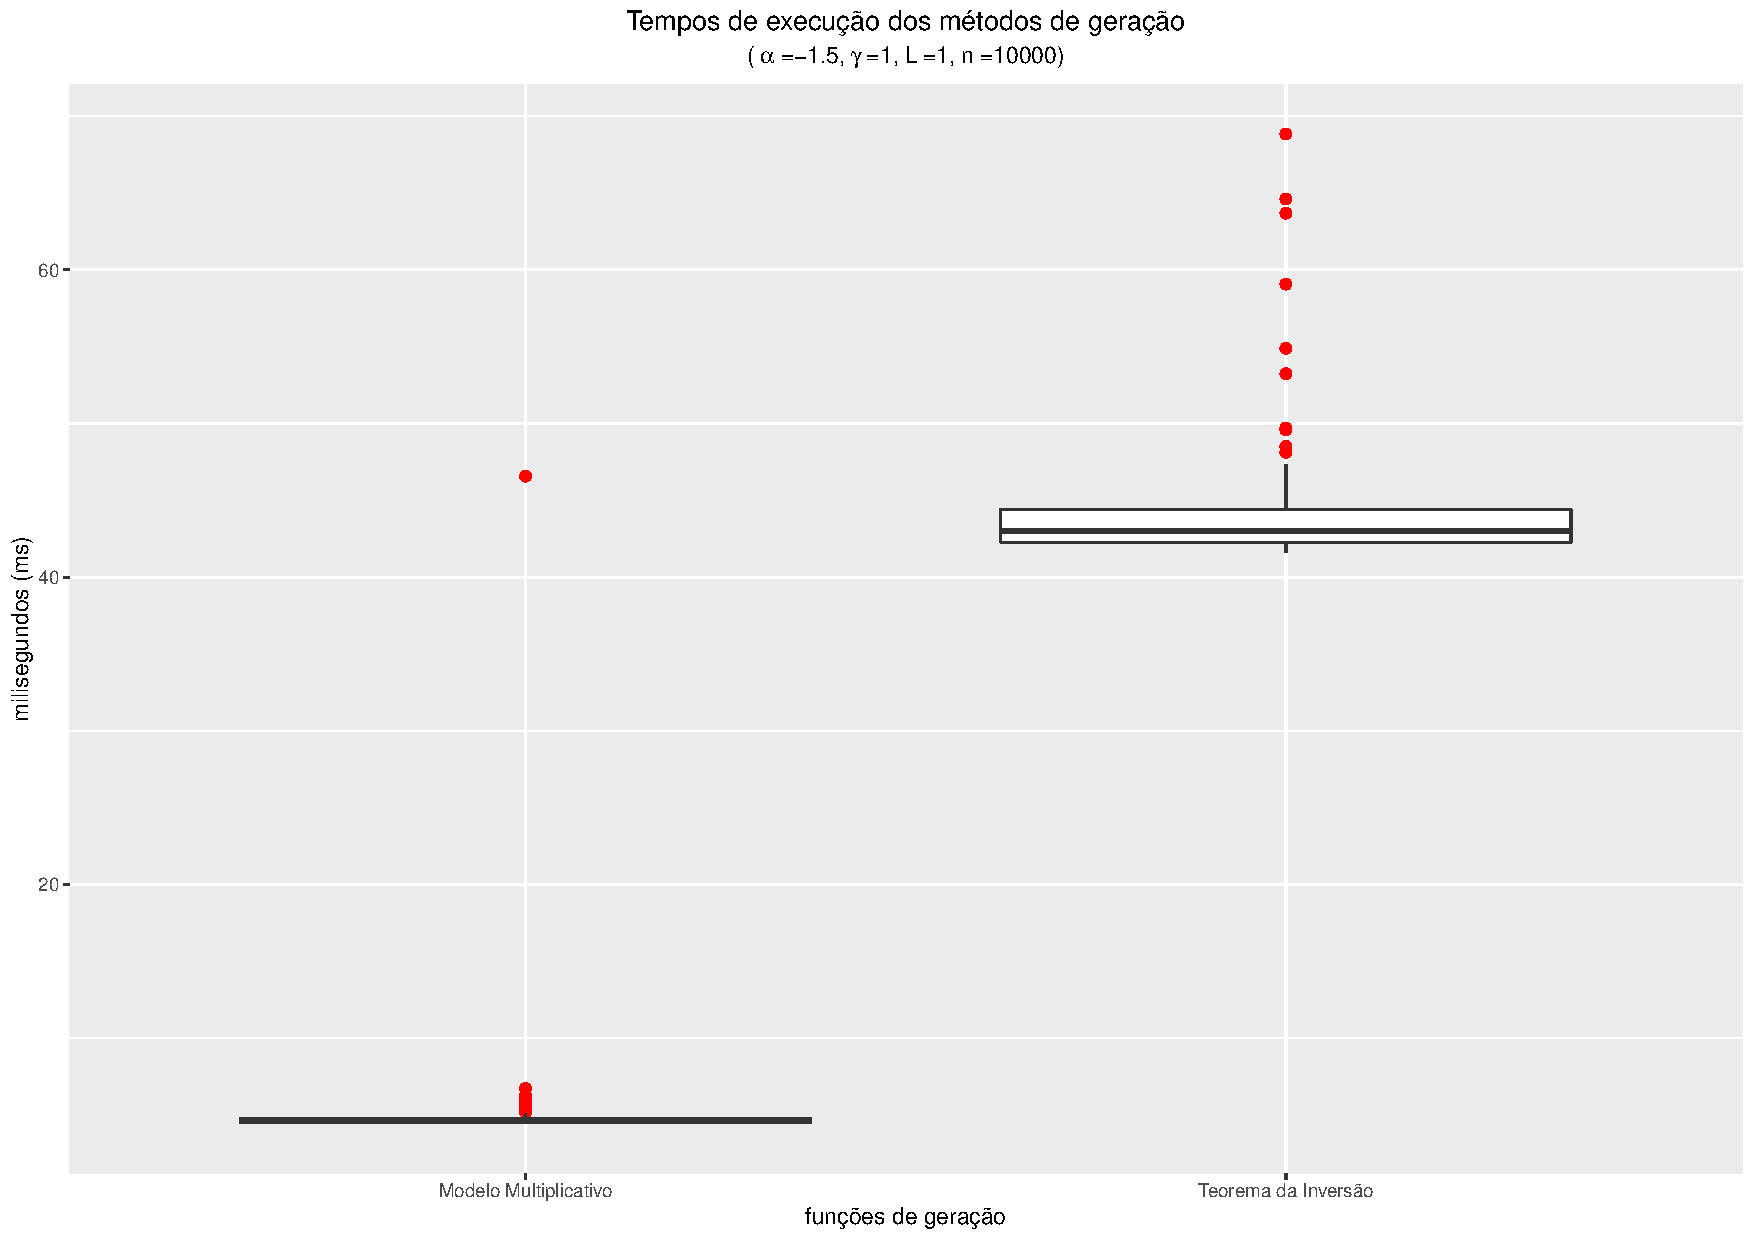
\includegraphics[scale=0.45]{plots/Runtime_1.pdf}
     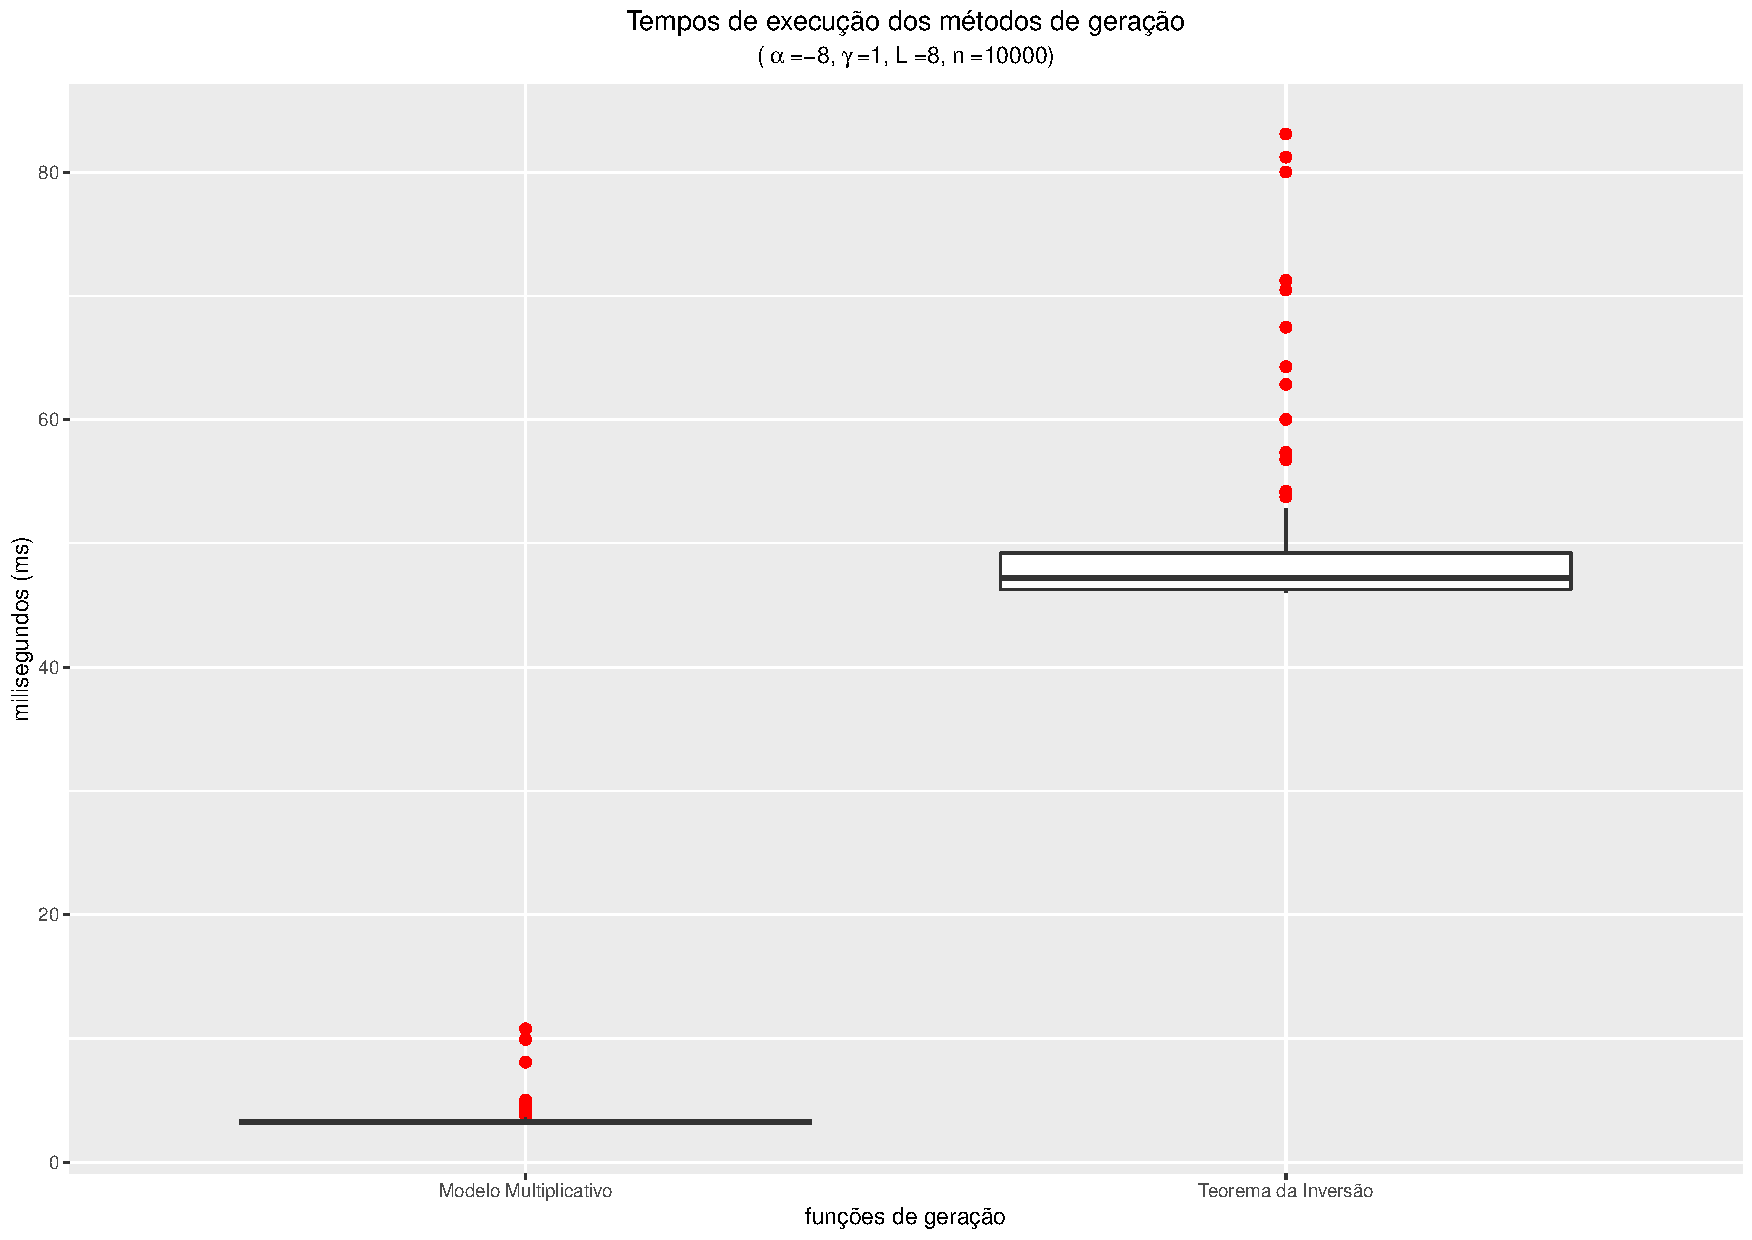
\includegraphics[scale=0.45]{plots/Runtime_2.pdf}
     \caption{Tempos de execução dos métodos de geração implementados}
     \label{graf_runtimes}
\end{figure}

Como pode-se perceber por meio da análise dos gráficos, o método de geração de variáveis aleatórias $G_I^0$ baseado no Modelo Multiplicativo obteve desempenho bem superior em termos de tempo de execução quando comparado com o Método baseado no Teorema da Inversão. No primeiro gráfico em que 10.000 amostras de variáveis aleatórias $G_I^0(-1.5, 1, 1)$ foram geradas, o Modelo Multiplicativo chegou a ser, em média, 9.5x mais rápido do que o Teorema da Inversão. Já no segundo gráfico em que o mesmo número de amostras foi utilizado e foram utilizados os parâmetros $G_I^0(-8, 1, 8)$ a vantagem desse método ficou ainda maior, alcançando a marca de aproximadamente 14x, em média, mais rápido. Para os demais casos testados, a vantagem do Modelo Multiplicativo prevaleceu.

Como conclusão, o Método de geração de variáveis aleatórias baseado no Modelo Multiplicativo foi utilizado no estudo de inferência desenvolvido no presente trabalho, visto que apresentou desempenho muito superior em todos os casos testados.

\section{Introdução ao Método de Monte Carlo}

De acordo com \citet{busto92}, experiências de Monte Carlo são uma poderosa técnica estatística usada para fornecer respostas aproximadas para questões sobre problemas complexos que podem incluir um componente estocástico, principalmente quando as técnicas analíticas e numéricas não fornecem, com uma quantidade aceitável de esforço, essas respostas de forma exata e completa. Estas técnicas de simulação são essencialmente baseadas em amostragem estatística controlada, e elas têm uma ampla gama de aplicações, incluindo, entre outras, mecânica estatística, biologia, jogos, otimização combinatória e engenharia.

Ainda segundo os autores, um estudo de simulação deve ser cuidadosamente planejado, a fim de obter resultados significativos e úteis. É comum, quando a simulação é usada, ter várias amostras para serem analisadas. Cada amostra poderia ter sido obtida, por exemplo, por simulações similares do mesmo sistema e com diferentes valores de parâmetros. Foi com base nessas ideias que os experimentos desenvolvidos neste trabalho foram realizados e os mesmos encontram-se descritos nas seções seguintes.

\section{Implementações dos Algoritmos de Estimação}

\subsection{Implementação do estimador de Máxima Verossimilhança}

Para a implementação do estimador de Máxima Verossimilhança foi proposto o uso do pacote \texttt{stats4} que disponibiliza a função \texttt{mle} que pode ser utilizada para se obter os estimadores de Máxima Verossimilhança tanto de distribuições populares, por exemplo, Gaussiana (\textit{Normal}), gama e t-Student, quanto de distribuições que não possuem implementação nativa na plataforma \texttt{R}.

Foi feita a implementação dos estimadores de MV para o modelo $G_I^0$ utilizando esse pacote. Nessa implementação, utilizou-se dados simulados gerados pelo gerador de variáveis aleatórias $G_I^0$ implementado a partir do Modelo Multiplicativo, onde as variáveis aleatórias são geradas a partir da razão de variáveis aleatórias gama.

Como nota-se na equação~\eqref{eq:mv}, capítulo~\ref{cap:fundamentacao}, a estimação por Máxima Verossimilhança consiste em encontrar um ponto que maximiza ($\arg\max$) a função de Verossimilhança e, com base nessa ideia, estamos diante de um problema de otimização. 
Um método utilizado para encontrar tais pontos de máximo é fazer como na equação dada em~\eqref{eq:gradient}, calculando as derivadas parciais e igualando a zero. 
Mas, como alternativa a isso, podemos aplicar diversos otimizadores existentes na literatura e que estão disponíveis para uso na função \texttt{mle} do pacote \texttt{stats4}.

Dentre os otimizadores disponíveis, talvez o mais utilizado deles seja o \emph{BFGS} é um método quasi-Newton (também conhecido como algoritmo de métrica variável).  
Esse algoritmo usa os valores da função e do seu gradientes para construir uma imagem da superfície a ser otimizada. 
Nas simulações construídas nesse trabalho utilizou-se o otimizador \emph{L-BFGS-B} de \citet{Byrd_1995} que permite restrições de limite, ou seja, cada variável que corresponde a um parâmetro da $G_I^0$ pode receber um limite inferior e/ou superior. 
Os valores buscados devem satisfazer as restrições do modelo. 
Ou seja, ele consiste de uma modificação de memória limitada do método \emph{BFGS} quasi-Newton que diminui o espaço de busca dos valores para os estimadores, sendo uma abordagem bem interessante para simulações com grande espaço de parâmetros.

\subsection{Implementação dos estimadores de Momentos e Log-Cumulantes}

Como já discutido, estimadores de Momentos são bastante utilizados nos processos de estimação de parâmetros para diversas distribuições. Nesse contexto, vale frisar que os estimadores de momentos fracionários foram amplamente utilizados com sucesso no trabalho de \citet{Clutter1997}. 
Com isso, utilizando-se $r = 1/2$ na equação dos momentos de ordem-$r$ dada em \eqref{eq:moments}, basta resolver no \texttt{R} a equação não linear dada em~\eqref{fractional_moments} que foi mostrada no fim da seção dos Estimadores de Momentos (capítulo ~\ref{cap:fundamentacao}) para obter o valor do estimador $\widehat{\alpha}$.

Sendo assim, o estimador de momentos foi implementado com o auxílio do pacote do \texttt{R} chamado \texttt{rootSolve}. 
Este foi criado para resolver os exemplos de análise de estabilidade e estado estacionário no livro de \citet{Soetaert2009}. Neste pacote, temos o método chamado \textit{uniroot} em que passamos a equação não linear desejada dada em~\eqref{fractional_moments} e, dessa forma, obteve-se de modo simples e prático o estimador $\widehat{\alpha}$.

De maneira análoga, os estimadores baseados no método de Log-Cumulantes (MLC) foram também encontrados de forma similar ao procedimento realizado para encontrar os estimadores de momentos. 
Mais uma vez, contou-se com o auxílio do pacote \texttt{rootSolve}, mais precisamente do método \emph{uniroot}, para calcular a raiz da equação não linear~\eqref{eq:alphaEst_logCum} dada no fim da seção dos Estimadores de Log-Cumulantes (capítulo~\ref{cap:fundamentacao}).

\subsection{Implementação do estimador de Distâncias Estocásticas}

Como já discutido anteriormente, para implementação dos estimadores obtidos pela Minimização de Distâncias Estocásticas foram necessárias duas etapas: 
1)~integração numérica necessária para calcular a distância Triangular entre a distribuição empírica e a densidade da $G_I^0$, e 
2)~otimização do sistema com relação ao parâmetro $\alpha$ de modo a encontrar o valor do parâmetro que minimiza a distância.

Nesse contexto, foi utilizado o pacote da plataforma \texttt{R} chamado \texttt{cubature} e, em especial, a função \texttt{adaptIntegrate} deste pacote para resolver a integral referente ao cálculo da distância Triangular. O algoritmo utilizado é uma integração multidimensional adaptativa sobre hipercubos. 
A minimização, por ser mais simples, foi feita sem o uso de funções auxiliares de pacotes existentes.

\section{Experimento I: Monte Carlo inicial}

Depois de implementados os algoritmos de estimação, um experimento inicial de Monte Carlo foi projetado para avaliar a acurácia e precisão (em relação ao valor real do parâmetro $\alpha$) de cada uma das técnicas no cálculo dos estimadores. 
O espaço de parâmetros utilizado consiste na grade formada pela tabela~\ref{tab:tabela_parameters}: 
variamos o parâmetro de textura $\alpha$ de modo a englobar a simulação de regiões extremamente texturizadas, de textura moderada e alvos sem textura. 
O parâmetro $n$, número de amostras, também foi variado de forma a representar amostras consideravelmente pequenas, médias e grandes. 
O parâmetro \textit{Looks} teve seu valor constante no experimento. 
Vale ressaltar que o valor $\gamma^{*}$, como foi dado em função do parâmetro $\alpha$ de modo a simplificar os cálculos de geração dos estimadores, não interferiu na simulação realizada.

\begin{table}[H]
\centering
\caption{Espaço de parâmetros utilizado na simulação inicial}
\sisetup{table-format = 3.2}
\label{tab:tabela_parameters}
\begin{tabular}{c|c}
\toprule 
\multicolumn{1}{c|}{Parâmetros} & \multicolumn{1}{c}{Valores}  \\ 
\midrule
\rowcolor[gray]{.9} 
$n$ & $\{200, 2000, 10000\}$ \\ \hline
$\alpha$ & $\{-2, -5, -8\}$ \\ \hline
\rowcolor[gray]{.9} $\gamma^{*}$ & $\{-\alpha - 1\}$ \\ \hline
\textit{Looks} & \{3\} \\ 
\bottomrule
\end{tabular}
\end{table}

Nesse experimento foi feito um total de 1000 replicações onde 1000 amostras foram geradas para cada ponto do espaço de parâmetros considerado na tabela anterior. Dessa forma, foi produzido o vetor de estimadores, $(\widehat{\alpha}_{1}, \widehat{\alpha}_{2}, \dots, \widehat{\alpha}_{1000})$ para cada valor do parâmetro $\alpha$ e para cada otimizador analisado. Com esses vetores em mãos, foram então calculados, para cada caso, a média das mil estimativas, $ \overline{\widehat{\alpha}} = (1000)^{-1} \sum_{i=1}^{1000} \widehat{\alpha_{i}} $, e o desvio padrão correspondente para medir a dispersão dos dados obtidos em torno da média. 

%%% ACF Evite "abaixo"
As tabelas~\ref{tab_maxver}, \ref{tab:mom}, \ref{tab:logcum} e \ref{tab:dt} mostram, respectivamente, os resultados dos estimadores de Máxima Verossimilhança, Momentos, Log-Cumulantes e Distâncias Estocásticas para o parâmetro $\alpha$ da $G_I^0$.

\begin{table}[H]
\centering
\caption{Estimadores de Máxima Verossimilhança} 
\begin{tabular}{@{\extracolsep{4pt}}c|c|c|c|c}
\toprule   
\multicolumn{1}{c}{\textbf{Amostras}} & \multicolumn{1}{c}{\textbf{Escala}} & \multicolumn{1}{c}{\textbf{Looks}} & \multicolumn{1}{c}{\textbf{Textura}} & \multicolumn{1}{c}{\textbf{Est. de Max. Ver.}} \\
 \cmidrule{1-1} 
 \cmidrule{2-2} 
 \cmidrule{3-3} 
 \cmidrule{4-4} 
 \cmidrule{5-5} 
\multicolumn{1}{c}{$n$} & \multicolumn{1}{c}{$\gamma$} & \multicolumn{1}{c}{$L$} & \multicolumn{1}{c}{$\alpha$} & \multicolumn{1}{c}{$\overline{\widehat{\alpha}}_{MV}$ (Desvio Padrão)} \\ 
\midrule
$200$  & $1$ & $3$ & $-2$ &  $-2.145$ ($0.234$) \\ 
   & $4$ & ~ & $-5$ &  $-5.453$ ($1.547$) \\ 
   & $7$ & ~ & $-8$ &  $-9.722$ ($7.014$) \\ \hline
$2000$  & $1$ & $3$ & $-2$ &  $-2.034$ ($0.056$)  \\ 
   & $4$ & ~ & $-5$ &  $-5.042$ ($0.372$)   \\
   & $7$ & ~ & $-8$ &  $-8.106$ ($0.877$)  \\ \hline
$10000$  & $1$ & $3$ & $-2$ & $-2.008$ ($0.026$)  \\ 
   & $4$ & ~ & $-5$ &  $-5.013$ ($0.143$)  \\
   & $7$ & ~ & $-8$ &  $-8.046$ ($0.339$)   \\
\bottomrule
\end{tabular}
\label{tab_maxver}
\end{table}

\begin{table}[H]
\centering
\caption{Estimadores de Momentos} 
\begin{tabular}{@{\extracolsep{4pt}}c|c|c|c|c}
\toprule   
\multicolumn{1}{c}{\textbf{Amostras}} & \multicolumn{1}{c}{\textbf{Escala}} & \multicolumn{1}{c}{\textbf{Looks}} & \multicolumn{1}{c}{\textbf{Textura}} & \multicolumn{1}{c}{\textbf{Est. de Momentos}} \\
 \cmidrule{1-1} 
 \cmidrule{2-2} 
 \cmidrule{3-3} 
 \cmidrule{4-4} 
 \cmidrule{5-5} 
\multicolumn{1}{c}{$n$} & \multicolumn{1}{c}{$\gamma$} & \multicolumn{1}{c}{$L$} & \multicolumn{1}{c}{$\alpha$} & \multicolumn{1}{c}{$\overline{\widehat{\alpha}}_{Mom12}$ (Desvio Padrão)} \\ 
\midrule
$200$  & $1$ & $3$ & $-2$ &  $-2.306$ ($1.172$) \\ 
   & $4$ & ~ & $-5$ &  $-5.486$ ($4.270$)\\ 
   & $7$ & ~ & $-8$ &  $-7.153$  ($4.040$) \\ \hline
$2000$  & $1$ & $3$ & $-2$ &  $-2.012$ ($0.129$) \\ 
   & $4$ & ~ & $-5$ &  $-5.410$ ($2.539$)  \\
   & $7$ & ~ & $-8$ &  $-9.404$ ($5.387$) \\ \hline
$10000$  & $1$ & $3$ & $-2$ & $-2.003$ ($0.055$) \\ 
   & $4$ & ~ & $-5$ &  $-5.105$ ($0.564$) \\
   & $7$ & ~ & $-8$ &  $-8.303$ ($1.633$)  \\
\bottomrule
\end{tabular}
\label{tab:mom}
\end{table}

\begin{table}[H]
\centering
\caption{Estimadores de Log-Cumulantes} 
\begin{tabular}{@{\extracolsep{4pt}}c|c|c|c|c}
\toprule   
\multicolumn{1}{c}{\textbf{Amostras}} & \multicolumn{1}{c}{\textbf{Escala}} & \multicolumn{1}{c}{\textbf{Looks}} & \multicolumn{1}{c}{\textbf{Textura}} & \multicolumn{1}{c}{\textbf{Est. Log-Cumulantes}} \\
 \cmidrule{1-1} 
 \cmidrule{2-2} 
 \cmidrule{3-3} 
 \cmidrule{4-4} 
 \cmidrule{5-5} 
\multicolumn{1}{c}{$n$} & \multicolumn{1}{c}{$\gamma$} & \multicolumn{1}{c}{$L$} & \multicolumn{1}{c}{$\alpha$} & \multicolumn{1}{c}{$\overline{\widehat{\alpha}}_{LCum}$ (Desvio Padrão)} \\ 
\midrule
$200$  & $1$ & $3$ & $-2$ &  $-2.040$ ($0.226$)\\ 
   & $4$ & ~ & $-5$ &  $-5.699$ ($3.360$)\\ 
   & $7$ & ~ & $-8$ &  $-6.506$ ($2.827$)\\ \hline
$2000$  & $1$ & $3$ & $-2$ &  $-2.006$  ($0.066$)\\ 
   & $4$ & ~ & $-5$ &  $-5.083$  ($0.678$) \\
   & $7$ & ~ & $-8$ &  $-8.371$ ($1.875$) \\ \hline
$10000$  & $1$ & $3$ & $-2$ & $-2.001$ ($0.027$) \\ 
   & $4$ & ~ & $-5$ &  $-5.022$ ($0.279$) \\
   & $7$ & ~ & $-8$ &  $-8.067$ ($0.740$)  \\
\bottomrule
\end{tabular}
\label{tab:logcum}
\end{table}

\begin{table}[H]
\centering
\caption{Estimadores de Distâncias Estocásticas} 
\begin{tabular}{@{\extracolsep{4pt}}c|c|c|c|c}
\toprule   
\multicolumn{1}{c}{\textbf{Amostras}} & \multicolumn{1}{c}{\textbf{Escala}} & \multicolumn{1}{c}{\textbf{Looks}} & \multicolumn{1}{c}{\textbf{Textura}} & \multicolumn{1}{c}{\textbf{Est. Distâncias Estocásticas}} \\
 \cmidrule{1-1} 
 \cmidrule{2-2} 
 \cmidrule{3-3} 
 \cmidrule{4-4} 
 \cmidrule{5-5} 
\multicolumn{1}{c}{$n$} & \multicolumn{1}{c}{$\gamma$} & \multicolumn{1}{c}{$L$} & \multicolumn{1}{c}{$\alpha$} & \multicolumn{1}{c}{$\overline{\widehat{\alpha}}_{DT}$ (Desvio Padrão)} \\ 
\midrule
$200$  & $1$ & $3$ & $-2$ &  $-2.031$ ($0.331$) \\ 
   & $4$ & ~ & $-5$ &  $-4.088$ ($1.385$)\\ 
   & $7$ & ~ & $-8$ &  $-5.594$ ($1.878$)\\ \hline
$2000$  & $1$ & $3$ & $-2$ &  $-1.334$ ($1.122$) \\ 
   & $4$ & ~ & $-5$ &  $-3.300$  ($0.803$) \\
   & $7$ & ~ & $-8$ &  $-5.730$ ($0.813$) \\ \hline
$10000$  & $1$ & $3$ & $-2$ & $-1.228$ ($0.196$) \\ 
   & $4$ & ~ & $-5$ &  $-3.360$ ($1.924$) \\
   & $7$ & ~ & $-8$ &  $-5.482$  ($2.765$) \\
\bottomrule
\end{tabular}
\label{tab:dt}
\end{table}

As figuras~\ref{graf_5}, \ref{graf_6} e \ref{graf_7} mostram uma comparação das estimativas providas pelas técnicas de estimação implementadas neste trabalho: Máxima Verossimilhança, Momentos, Log-Cumulantes e Distâncias Estocásticas. Nas figuras seguintes, "MLE" denota os estimadores baseados em Máxima Verossimilhança (do inglês, \textbf{M}aximum \textbf{L}ikelihood \textbf{E}stimation). Os tamanhos de amostra estão nas abscissas (eixo-x), e estão apresentadas em escala logarítmica para melhor visualização. As estimativas da média são apresentadas com barras de erro que exibem o intervalo de confiança baseado na distribuição Gaussiana com nível de confiança de \SI{95}{\percent}.

\begin{figure}[H]
     \centering
     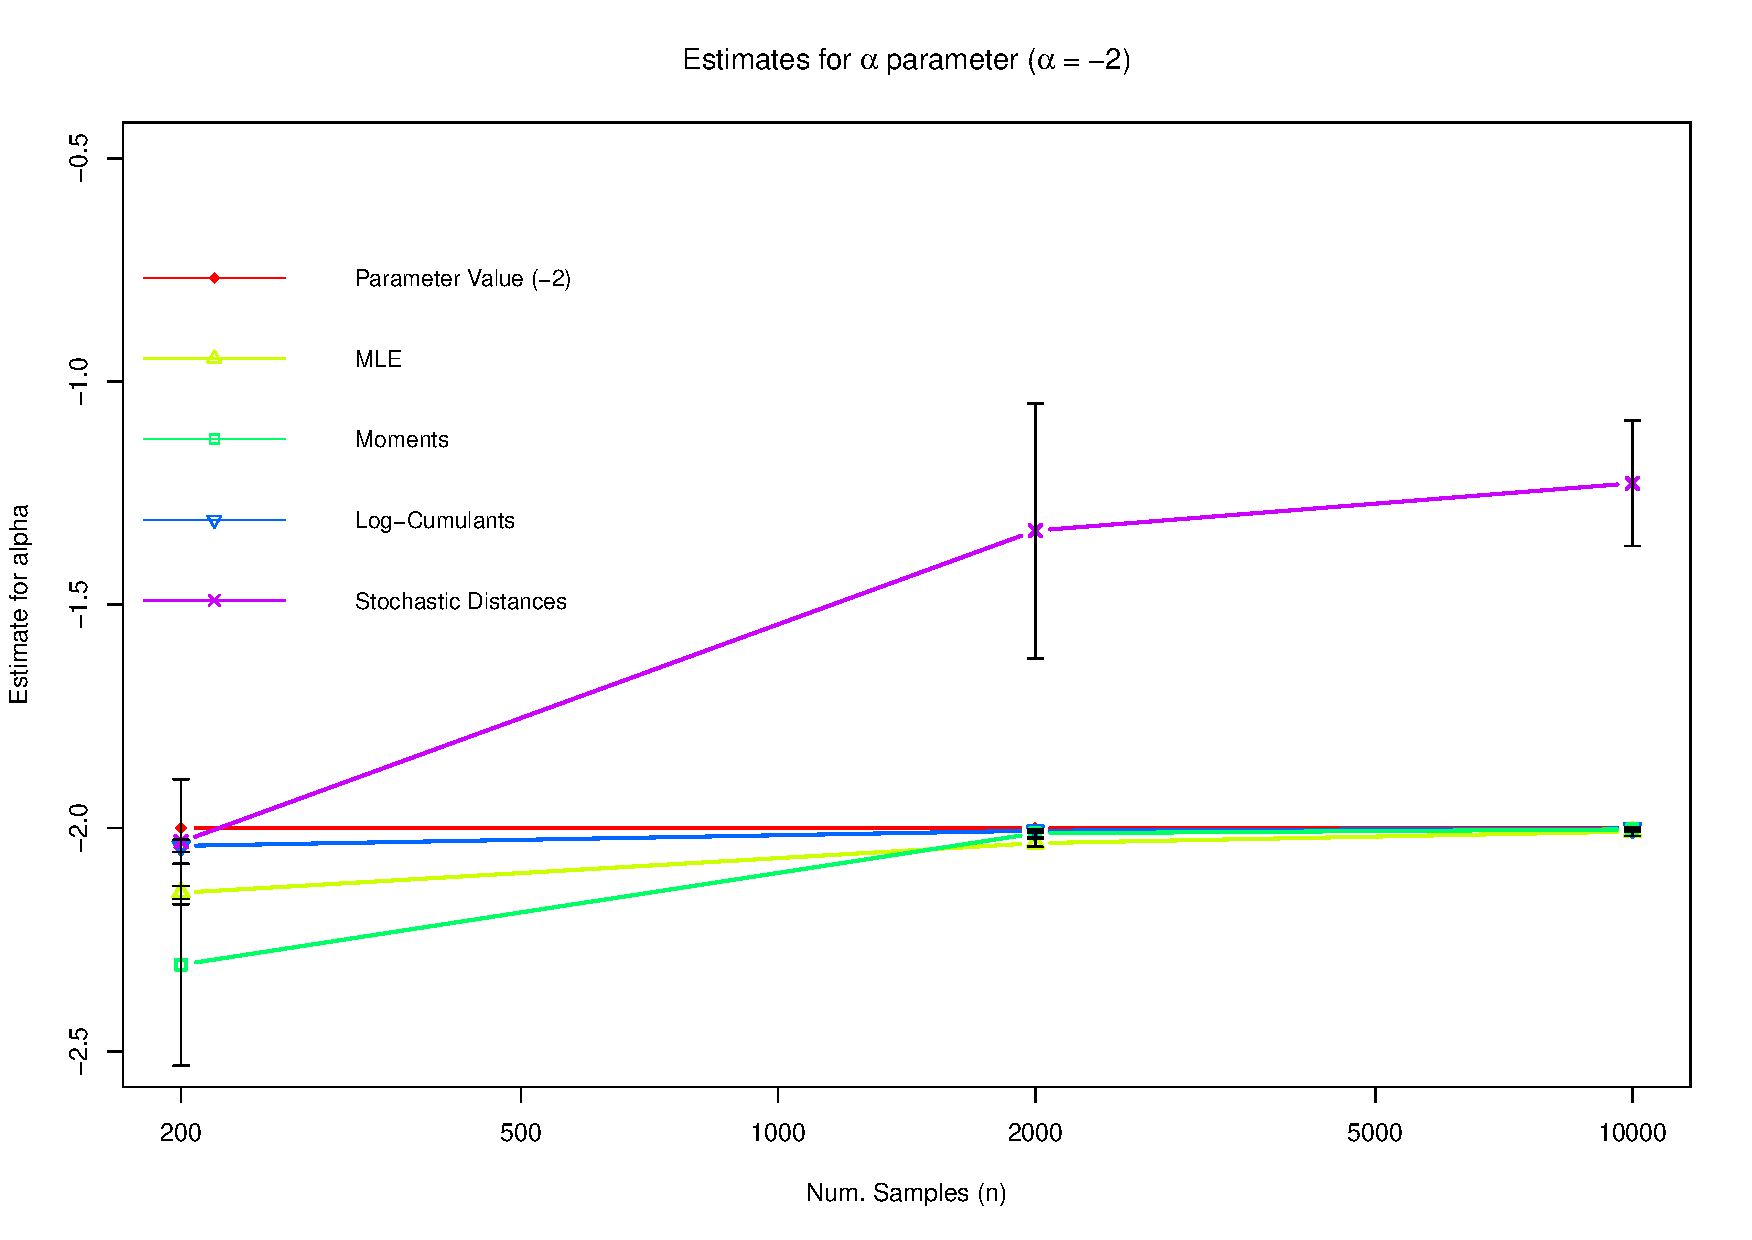
\includegraphics[scale=0.5]{plots/ComparisonAlpha-2.pdf}
     \caption{Estimativas obtidas para o parâmetro $\alpha = -2$}
     \label{graf_5}
\end{figure}
\begin{figure}[H]
     \centering
     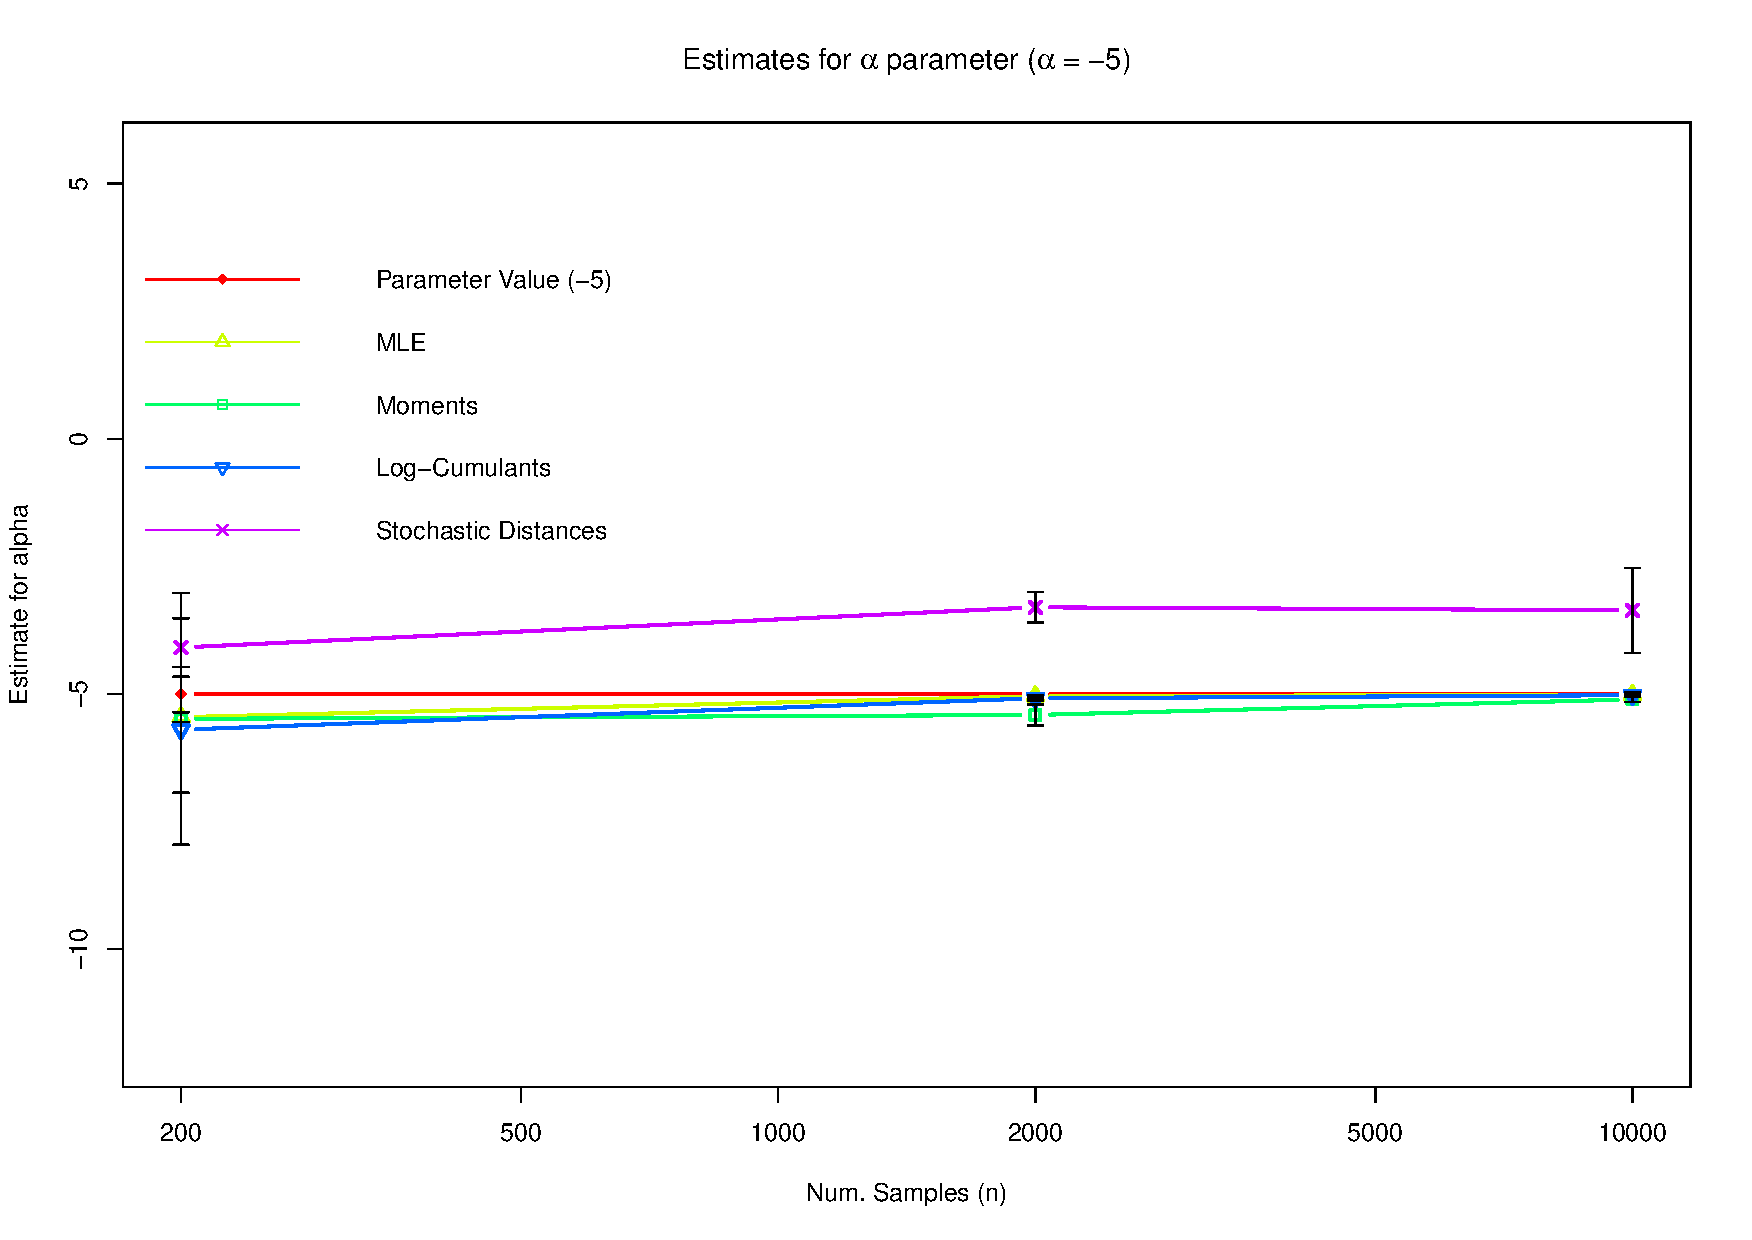
\includegraphics[scale=0.5]{plots/ComparisonAlpha-5.pdf}
     \caption{Estimativas obtidas para o parâmetro $\alpha = -5$}
     \label{graf_6}
\end{figure}
\begin{figure}[H]
     \centering
     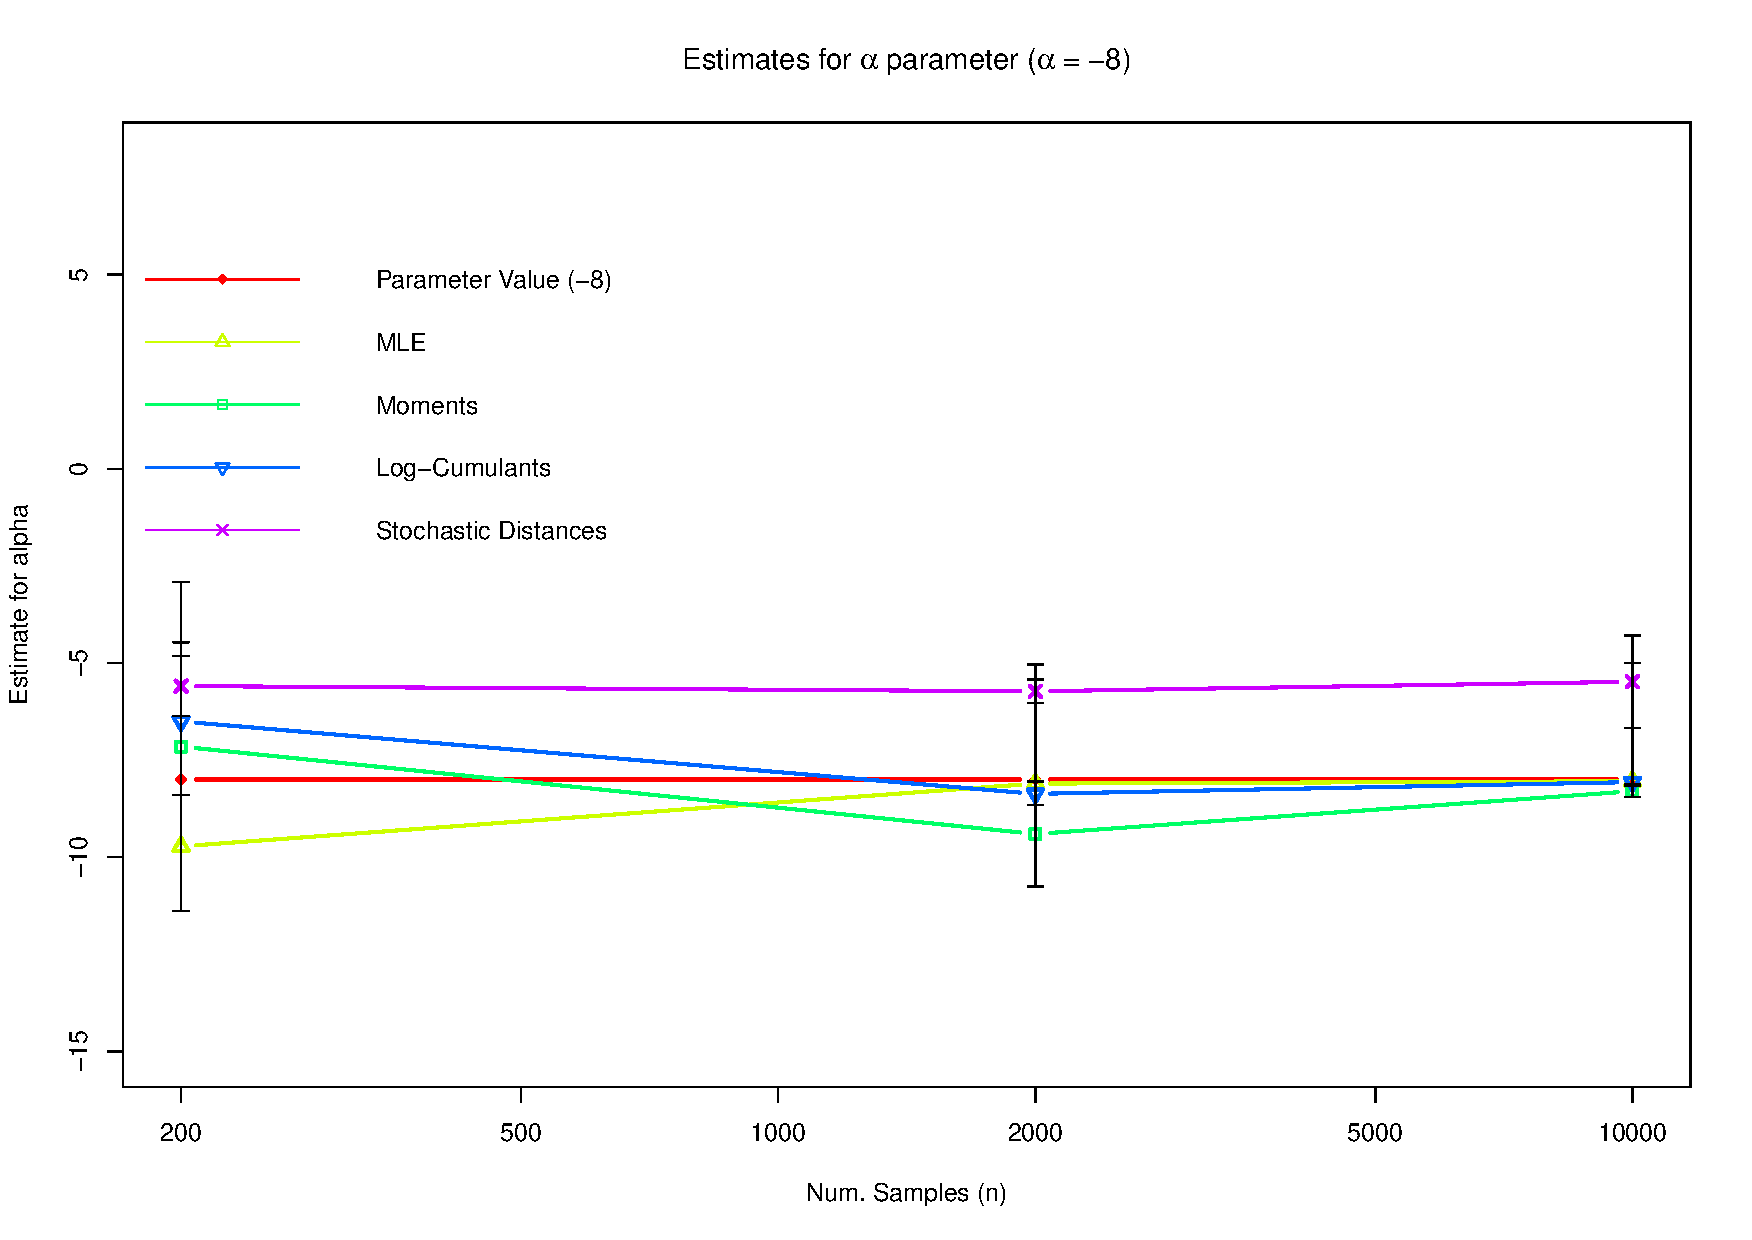
\includegraphics[scale=0.5]{plots/ComparisonAlpha-8.pdf}
     \caption{Estimativas obtidas para o parâmetro $\alpha = -8$}
     \label{graf_7}
\end{figure}

Para o estudo inicial de simulação feito, pode-se perceber através dos gráficos que os métodos de estimação conquistaram resultados satisfatórios. Em análise aos gráficos, os métodos baseados em Máxima Verossimilhança e Log-Momentos apresentaram boa capacidade de convergência para o verdadeiro valor do parâmetro à medida que o número de amostras (tamanho amostral) aumentou. No entanto, sempre pode existir uma eventual falta de convergência para alguns valores do parâmetro inerente a todos os algoritmos de estimação implementados. 
O estimador baseado em mecanismos da Teoria da Informação, mas especificamente na Minimização de Distâncias Estocásticas, foi o que apresentou resultados mais discrepantes em relação aos demais métodos em análise aos gráficos gerados.

Entretanto, este foi apenas um estudo inicial a respeito das técnicas de estimação de parâmetros implementadas e  novos planos de simulação e investigação mais elaborados foram feitos para avaliar melhor tais técnicas, bem como analisar suas possíveis restrições e aplicações em um contexto unificado, onde existirá uma rotina de estimação geral que engloba esses métodos e seja capaz de aplicar os mais adequados para cada situação com a mínima intervenção possível do usuário tendo em vista seus pontos fortes e fracos de aplicação.

\section{Experimento II: Monte Carlo mais elaborado}

Agora nessa seção será descrito o segundo experimento de Monte Carlo que foi construído de forma mais minuciosa e elaborada de modo a possibilitar uma análise mais profunda acerca das técnicas de estimação implementadas. 
Nesse contexto, temos a tabela~\ref{tab:tabela_parameters_2} contendo o espaço de parâmetros utilizado nesta simulação.

\begin{table}[H]
\centering
\caption{Espaço de parâmetros utilizado na simulação mais elaborada}
\smallskip
\sisetup{table-format = 3.2}
\label{tab:tabela_parameters_2}
\begin{tabular}{c|c}
\toprule 
\multicolumn{1}{c|}{Parâmetros} & \multicolumn{1}{c}{Valores}  \\ 
\midrule
\rowcolor[gray]{.9} 
$n$ & $\{30, 100, 1000\}$ \\ \hline
$\alpha$ & $\{-1.5, -3, -8\}$ \\ \hline
\rowcolor[gray]{.9} $\gamma^*$ & $\{-\alpha - 1\}$ \\ \hline
\textit{Looks} & $\{1, 3, 5, 8\}$ \\ 
\bottomrule
\end{tabular}
\end{table}

Para realizar este experimento de Monte Carlo levou-se em consideração que amostras maiores apresentam menor variabilidade de dados em comparação com amostrar menores, então no contexto das replicações existentes no experimento definiu-se uma constante $R = 100.000$ onde o número de réplicas/repetições de amostras é dado conforme a seguinte fórmula:
\begin{equation}
    Rep = [R/n]. \label{eq:rep}
\end{equation}
Assim, o número de replicações varia de acordo com cada tamanho de amostra em que amostras menores precisam ser replicadas um número maior de vezes para possibilitar a coleta de maior variabilidade dos dados, enquanto que amostras maiores não necessariamente precisam ser replicadas um número grande de vezes como no caso das amostras menores, sendo suficiente apenas um número de replicações inferior. 

Desta maneira, os estimadores foram gerados com base nesse experimento. A estimativa do viés, denotada por $\widehat{B}(\widehat{\alpha}) = \overline{\widehat{\alpha_i}} - \alpha$, 
%%% ACF Diferencie o viés teórico da estimativa do viés. A equação acima está errada para ambos.
e o erro quadrático médio foram calculados e comparados para análise da acurácia. Nas figuras seguintes, "ML", "Mom", "LCum" e "DT" denotam os estimadores baseados em Máxima Verossimilhança (do inglês, \textbf{M}aximum \textbf{L}ikelihood), Momentos, Log-Cumulantes e Distância Triangular. Os tamanhos amostrais se encontram nas abscissas dos gráficos e, para uma melhor visualização, estão apresentados em uma escala logarítmica. O valor real do parâmetro está presente em cada gráfico representado pela linha de cor vermelha. Abaixo estão os gráficos gerados agrupados pelo número de \textit{Looks}.
\begin{figure}[H]
     \centering
     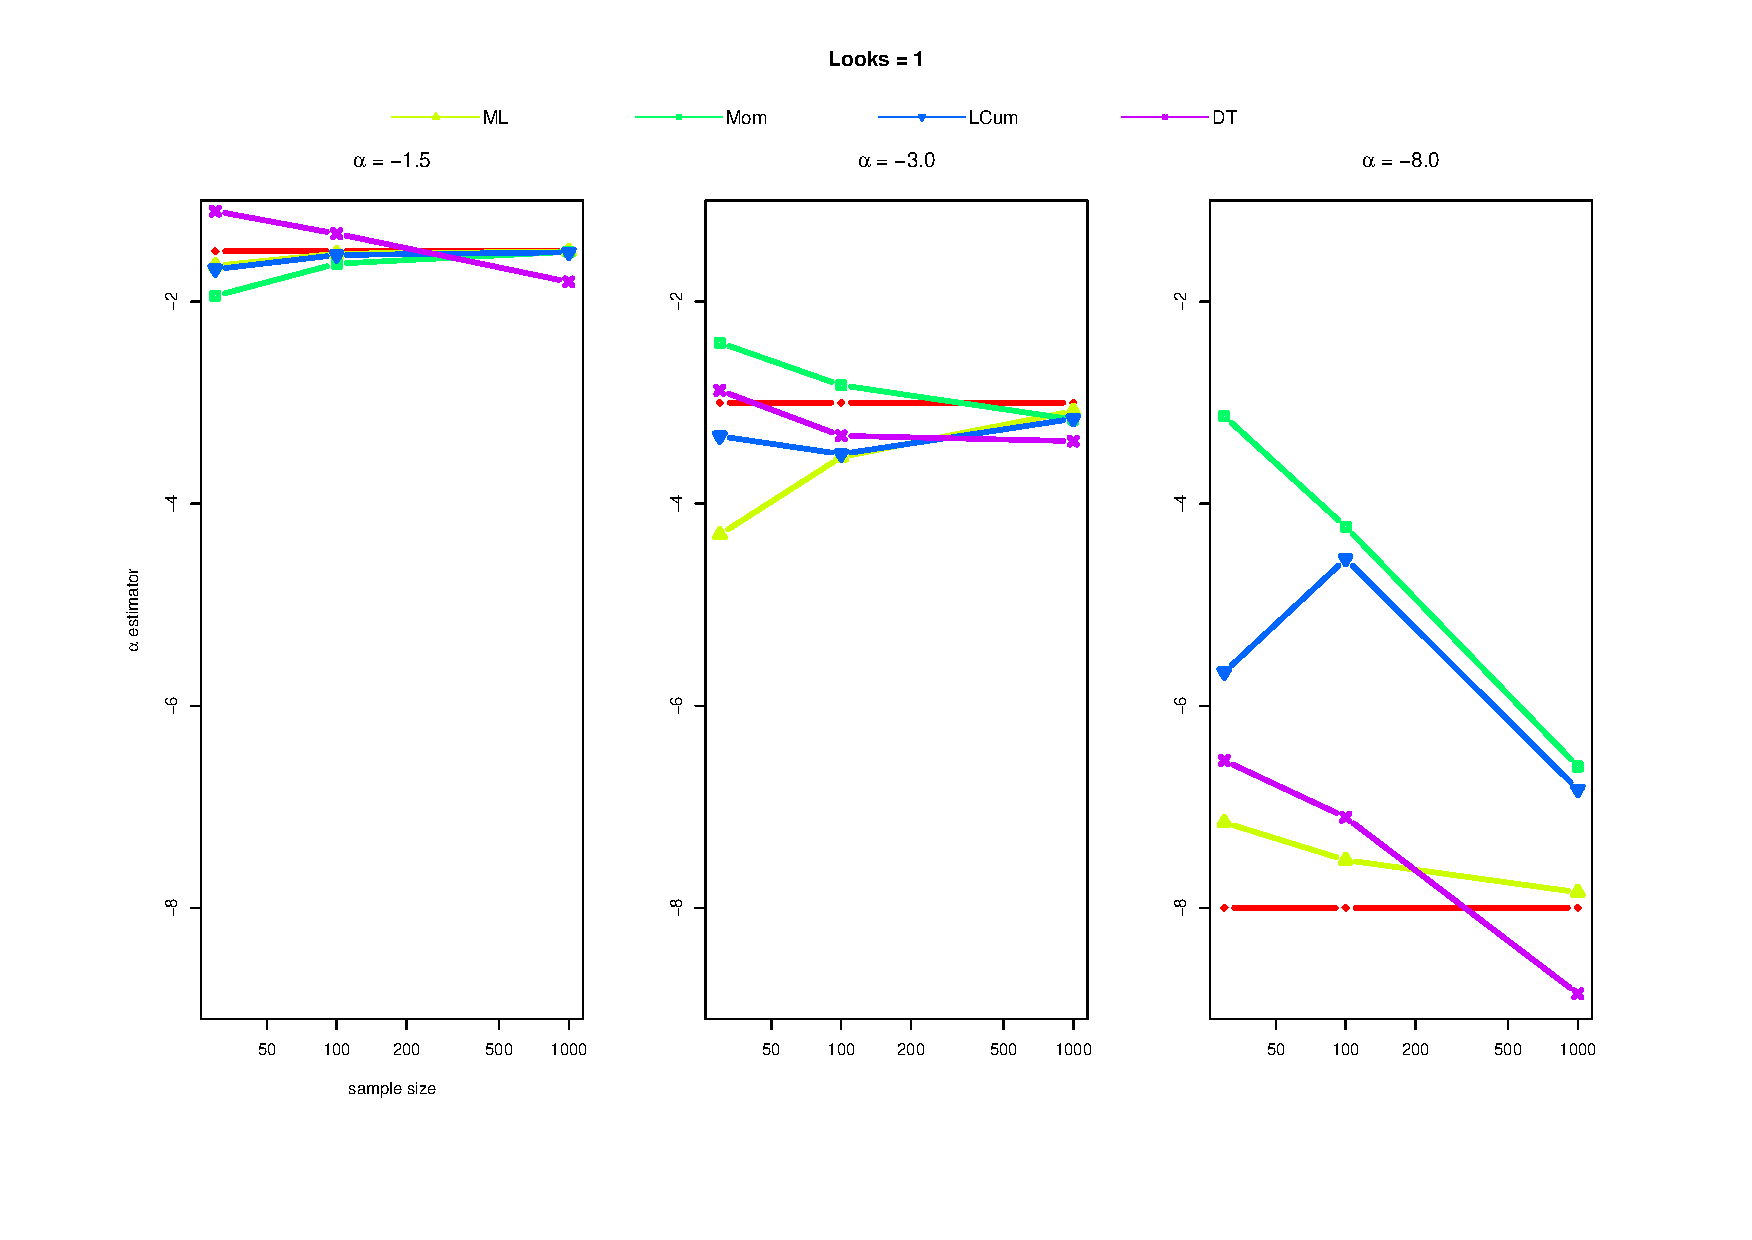
\includegraphics[scale=0.5]{plots/estimators_L=1.pdf}
     \caption{Estimativas obtidas para $L=1$}
     \label{graf_8}
\end{figure}
\begin{figure}[H]
     \centering
     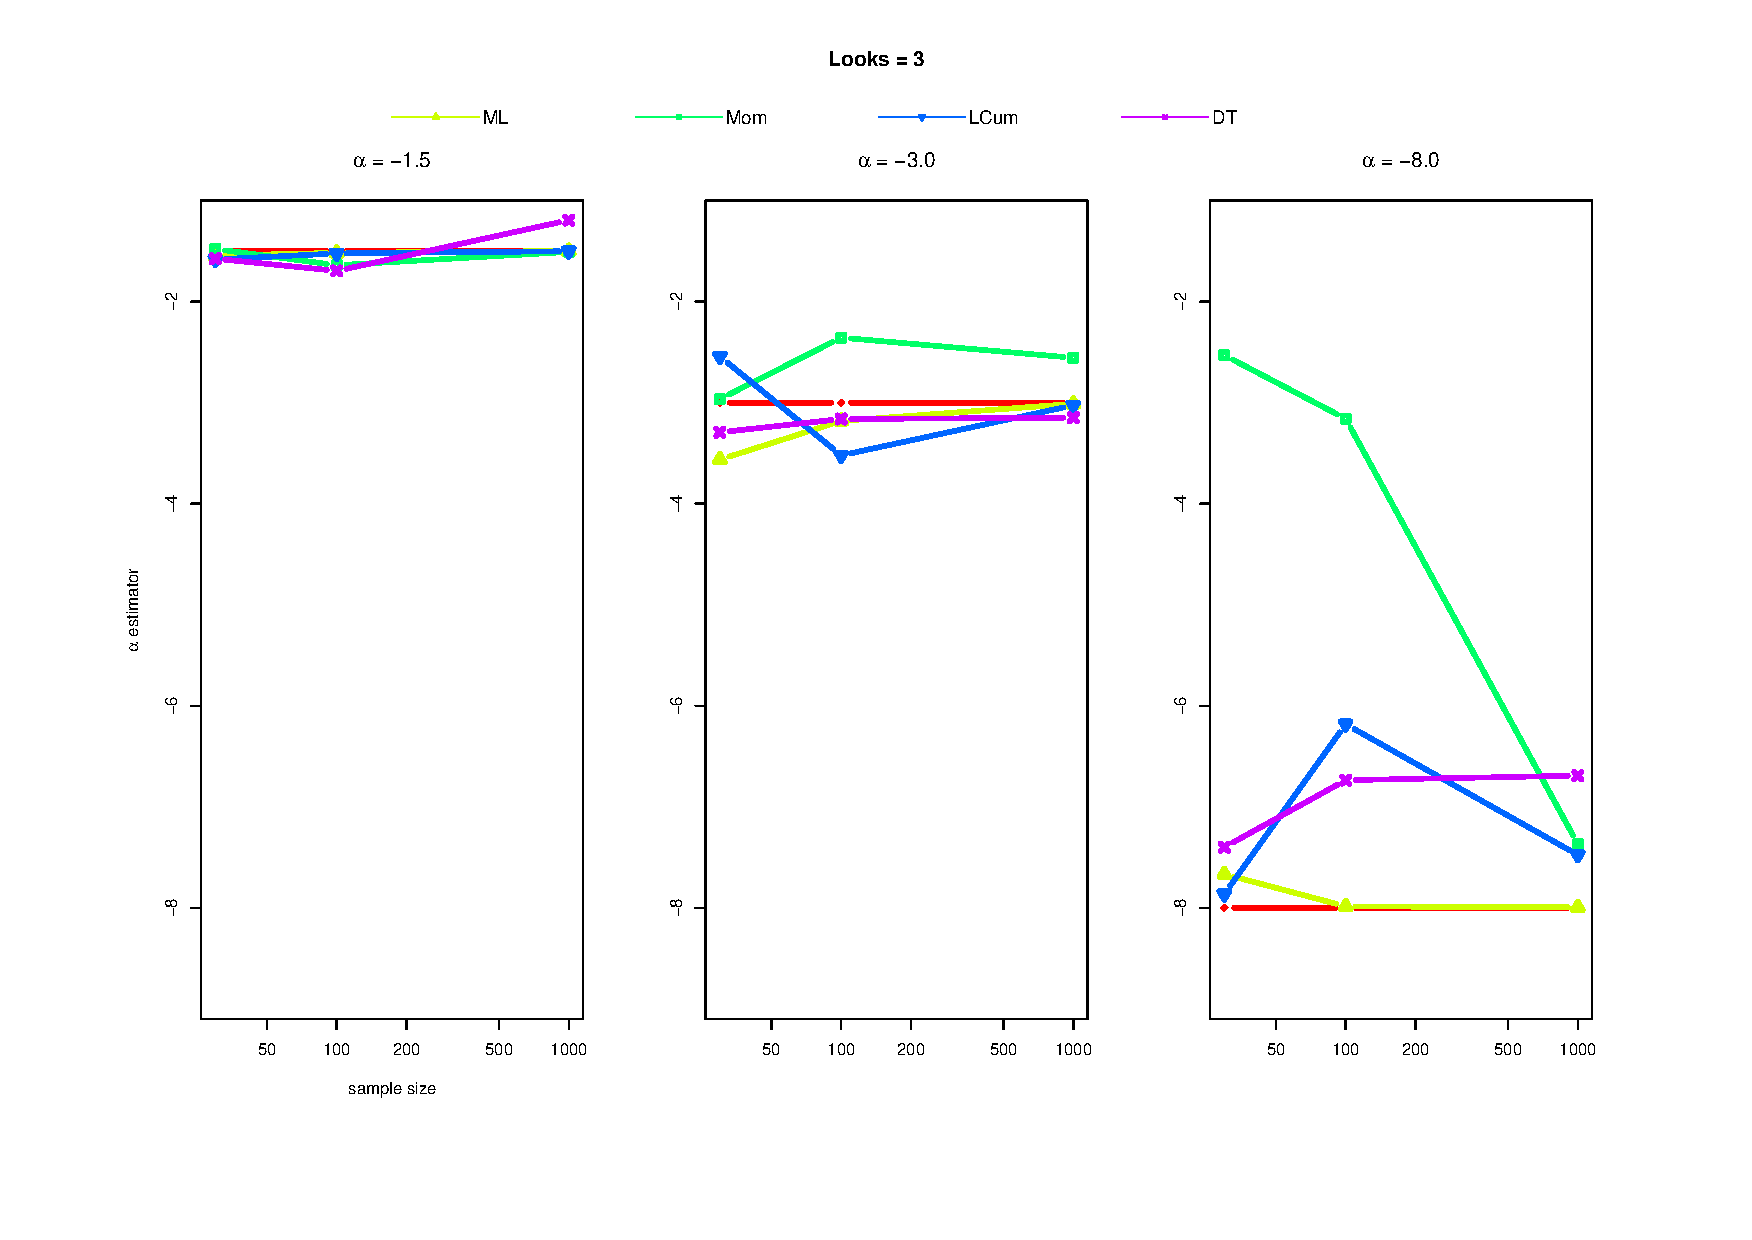
\includegraphics[scale=0.5]{plots/estimators_L=3.pdf}
     \caption{Estimativas obtidas para $L=3$}
     \label{graf_9}
\end{figure}
\begin{figure}[H]
     \centering
     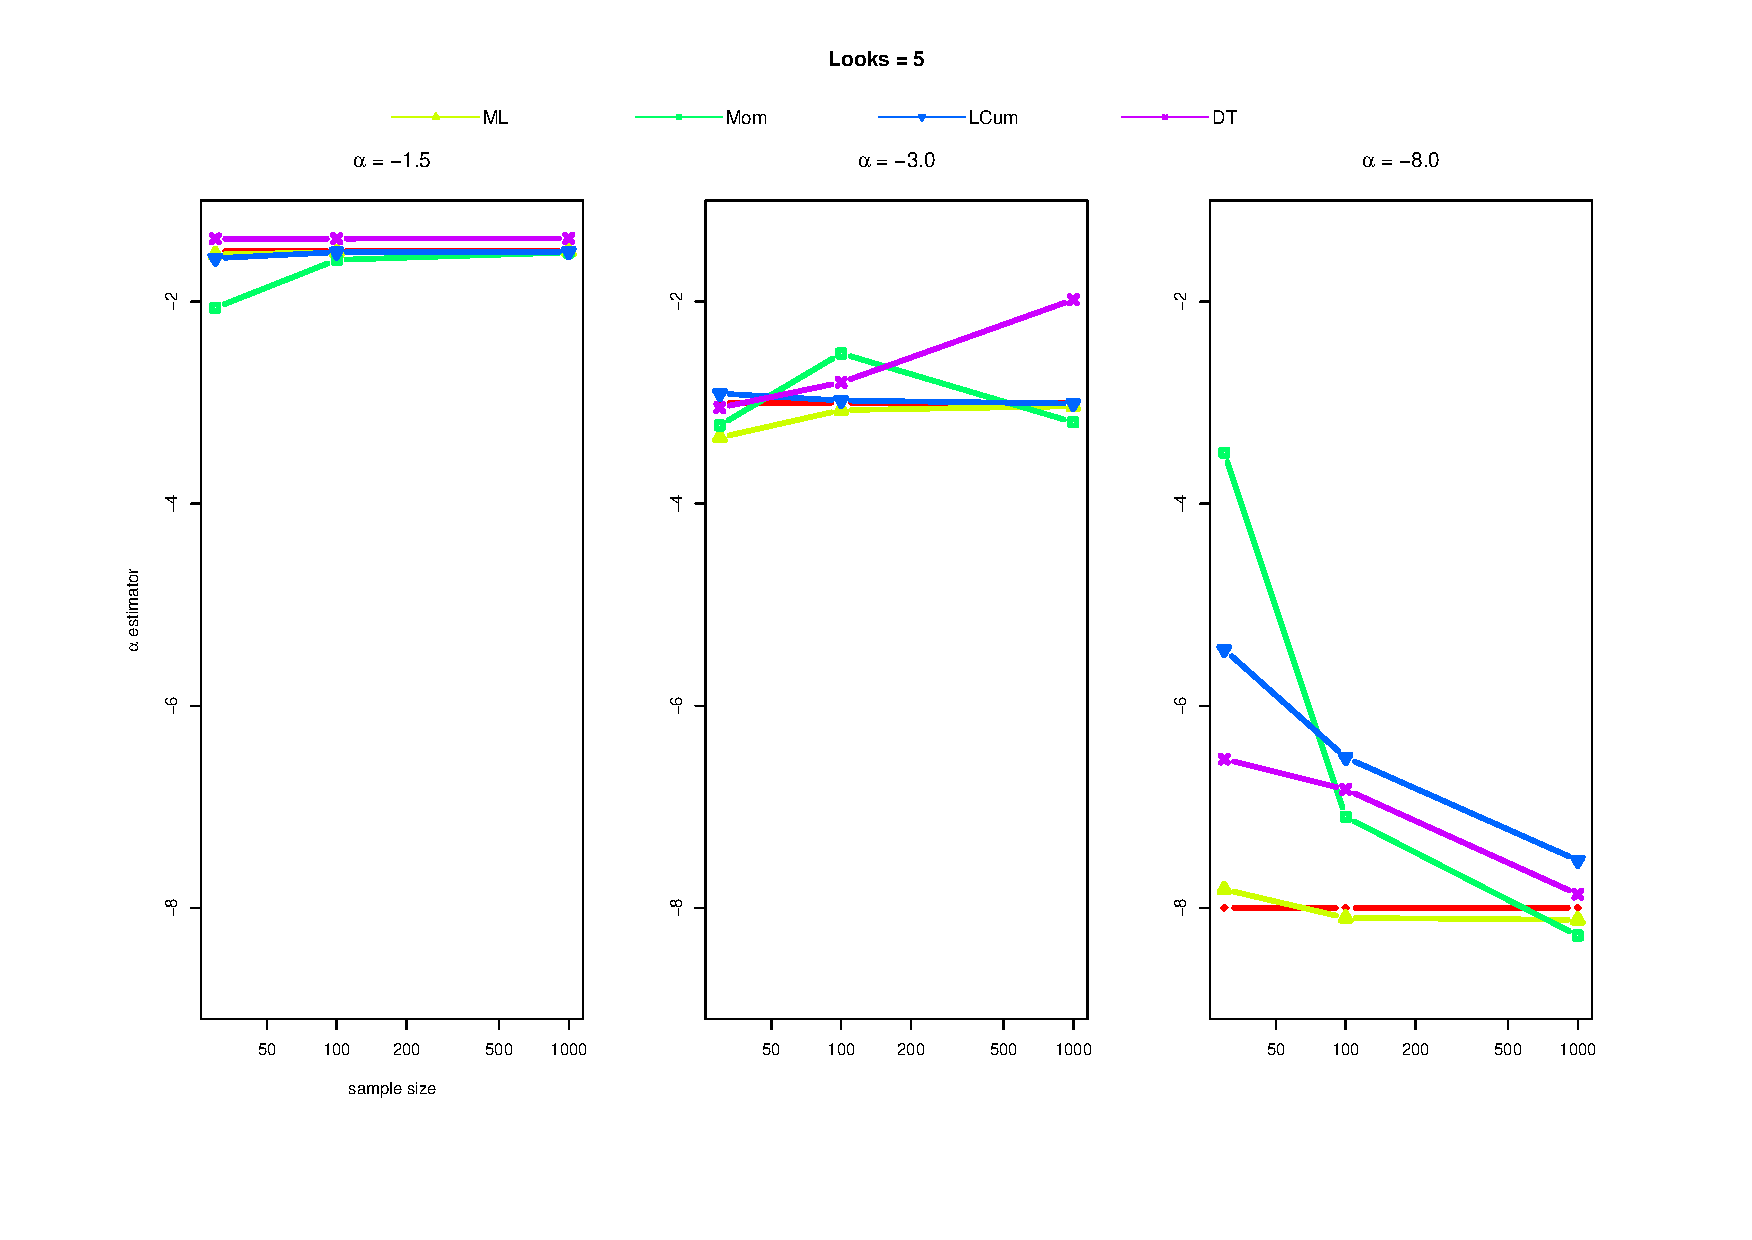
\includegraphics[scale=0.5]{plots/estimators_L=5.pdf}
     \caption{Estimativas obtidas para $L=5$}
     \label{graf_10}
\end{figure}
\begin{figure}[H]
     \centering
     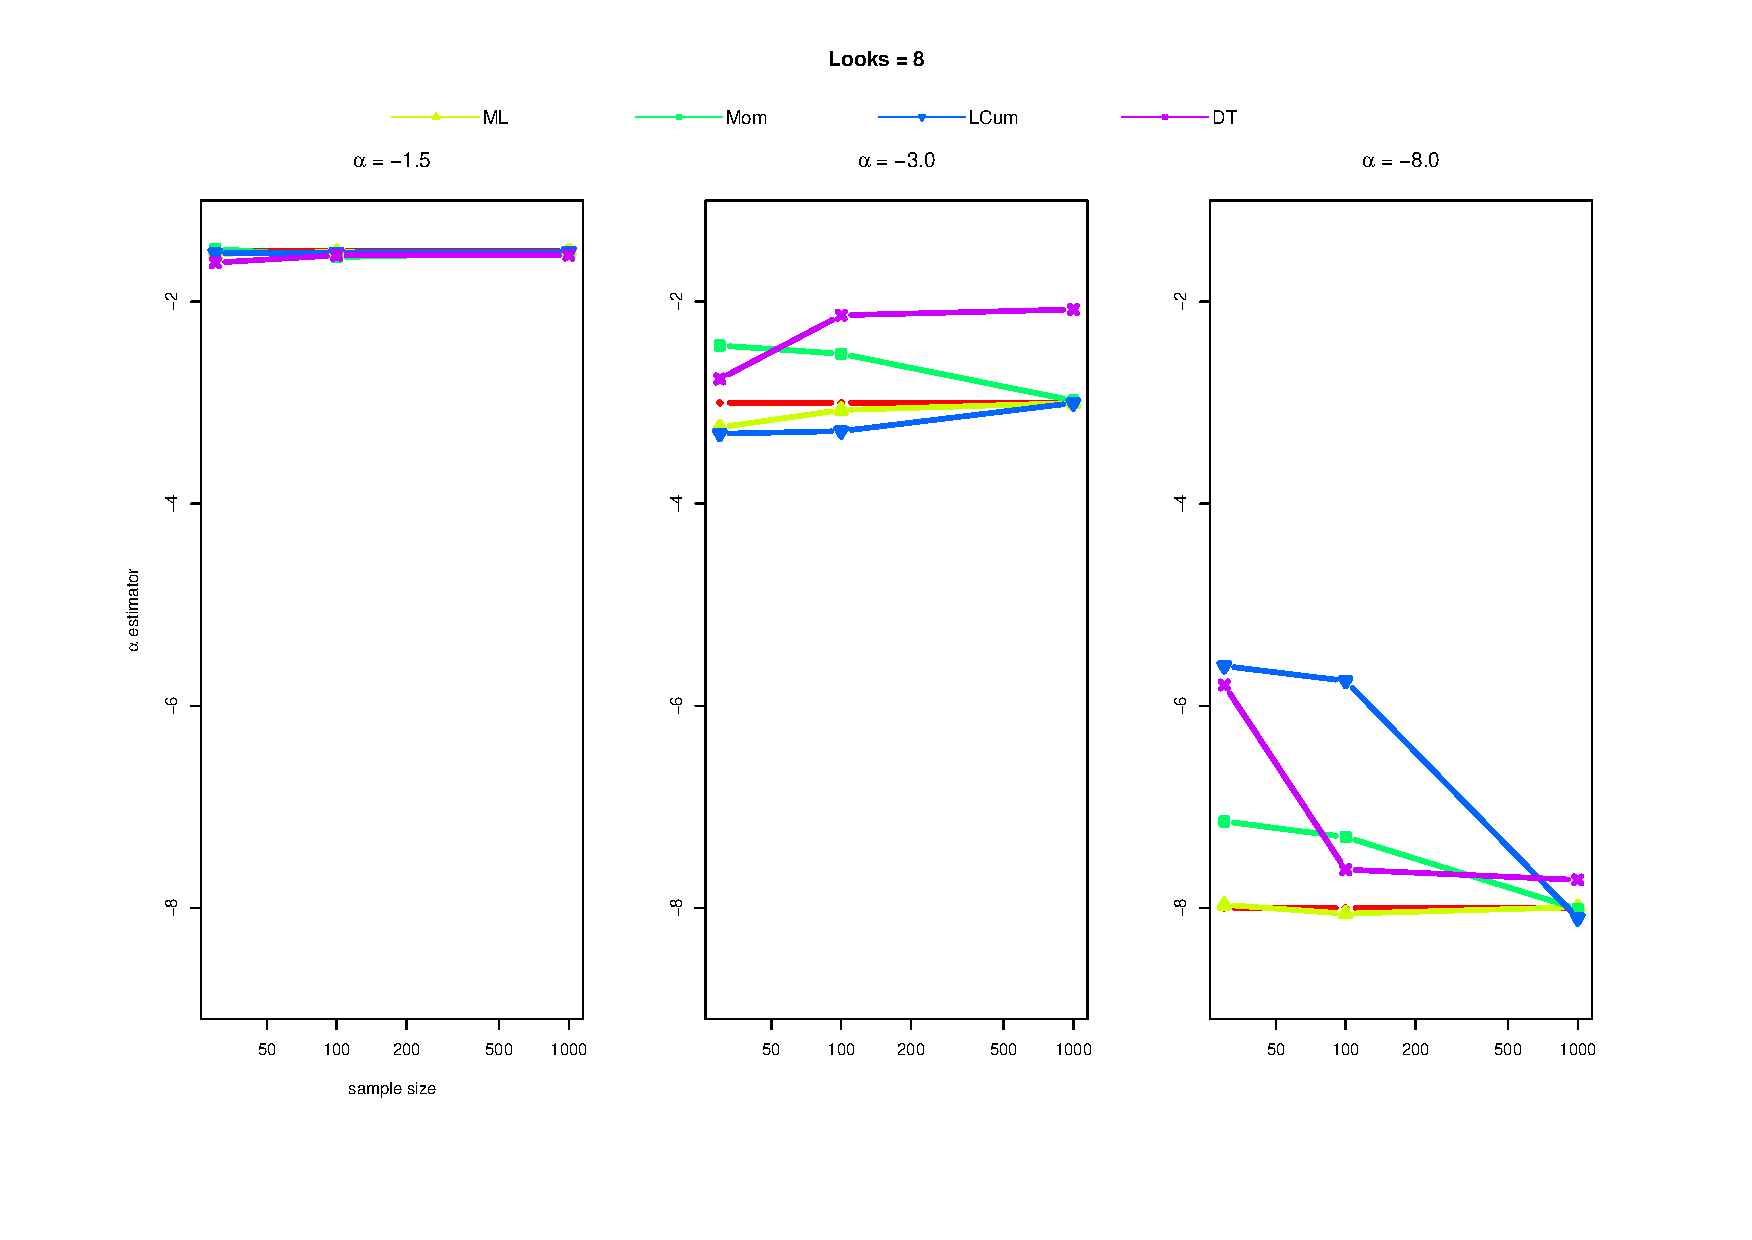
\includegraphics[scale=0.5]{plots/estimators_L=8.pdf}
     \caption{Estimativas obtidas para $L=8$}
     \label{graf_11}
\end{figure}

As figuras~\ref{graf_12}, \ref{graf_13}, \ref{graf_14} e \ref{graf_15} são relativas aos erros quadráticos médios que foram calculados durante a experiência de Monte Carlo realizada. 
\begin{figure}[H]
     \centering
     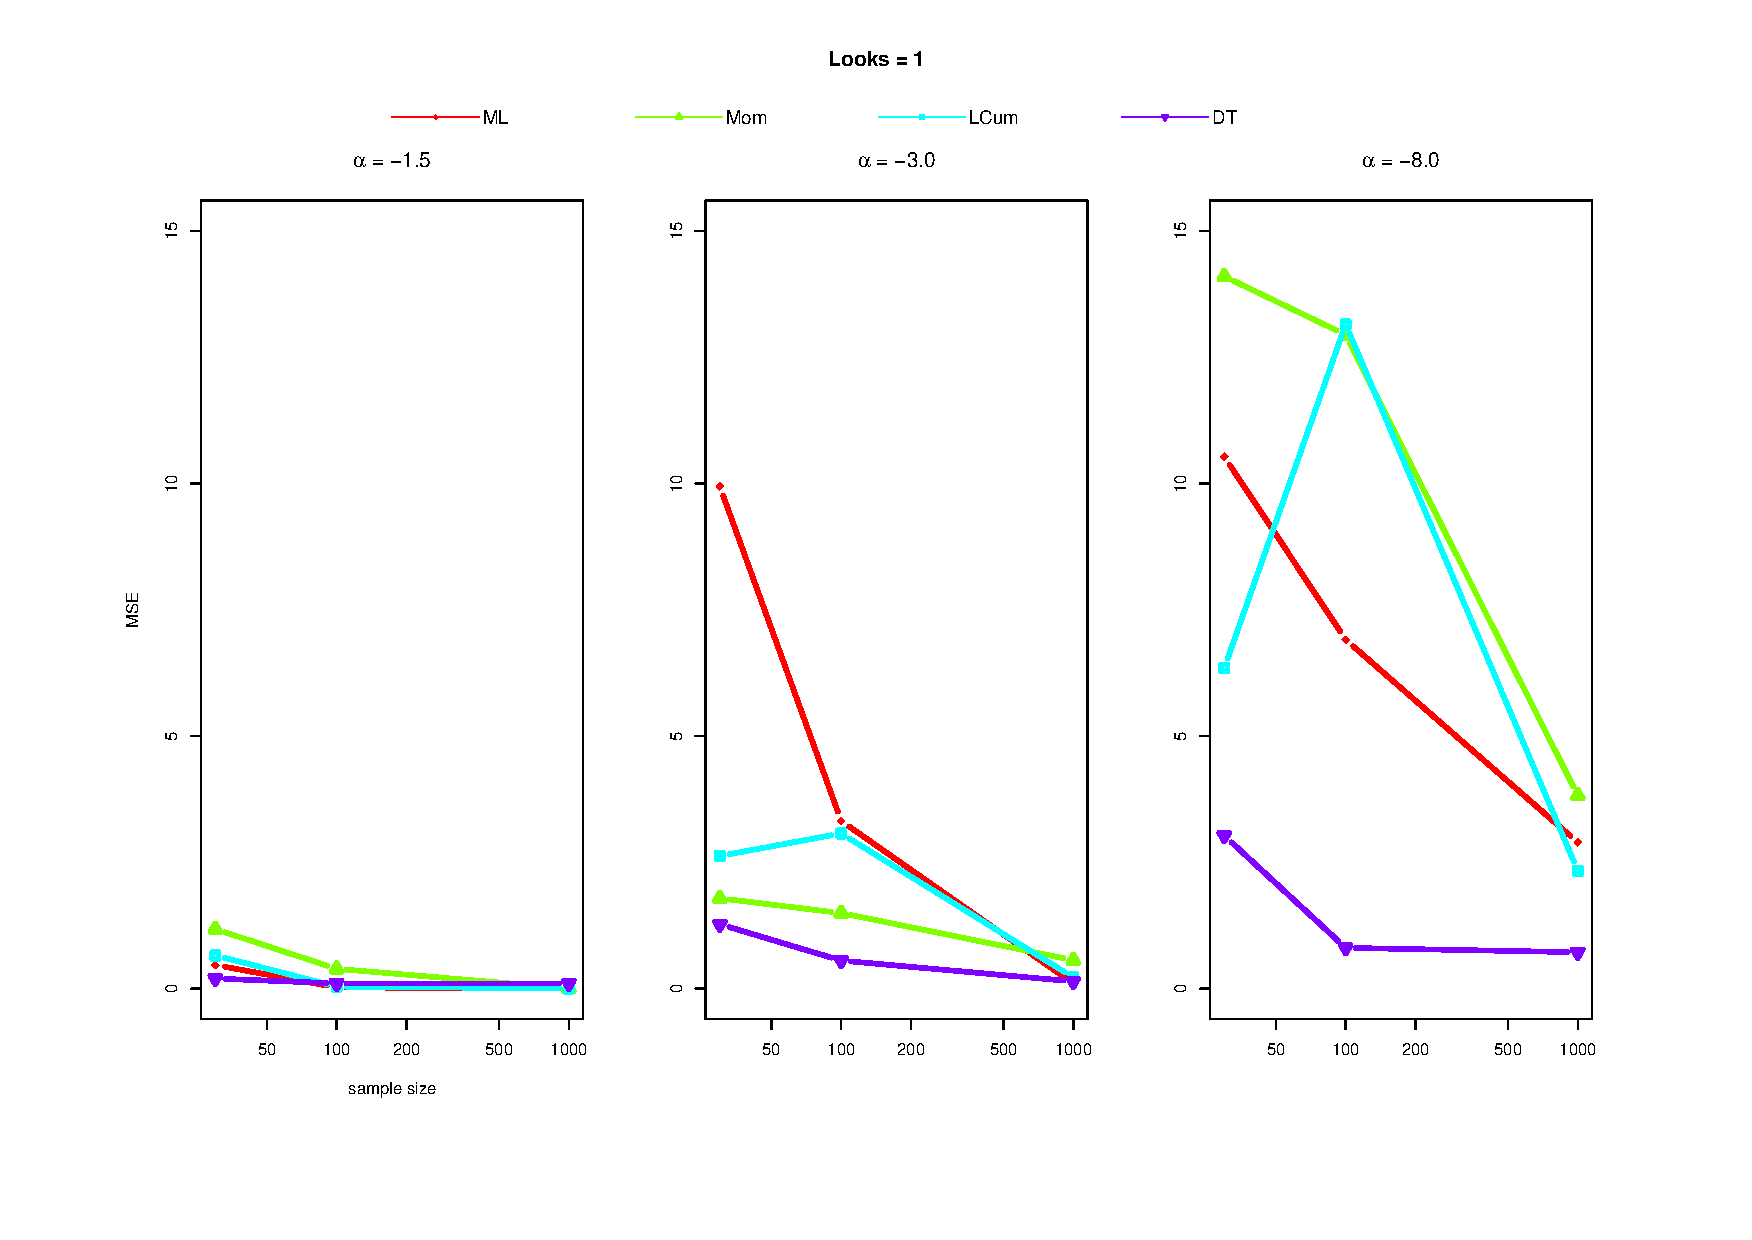
\includegraphics[scale=0.45]{plots/mse_L=1.pdf}
     \caption{Erros obtidos para $L=1$}
     \label{graf_12}
\end{figure}
\begin{figure}[H]
     \centering
     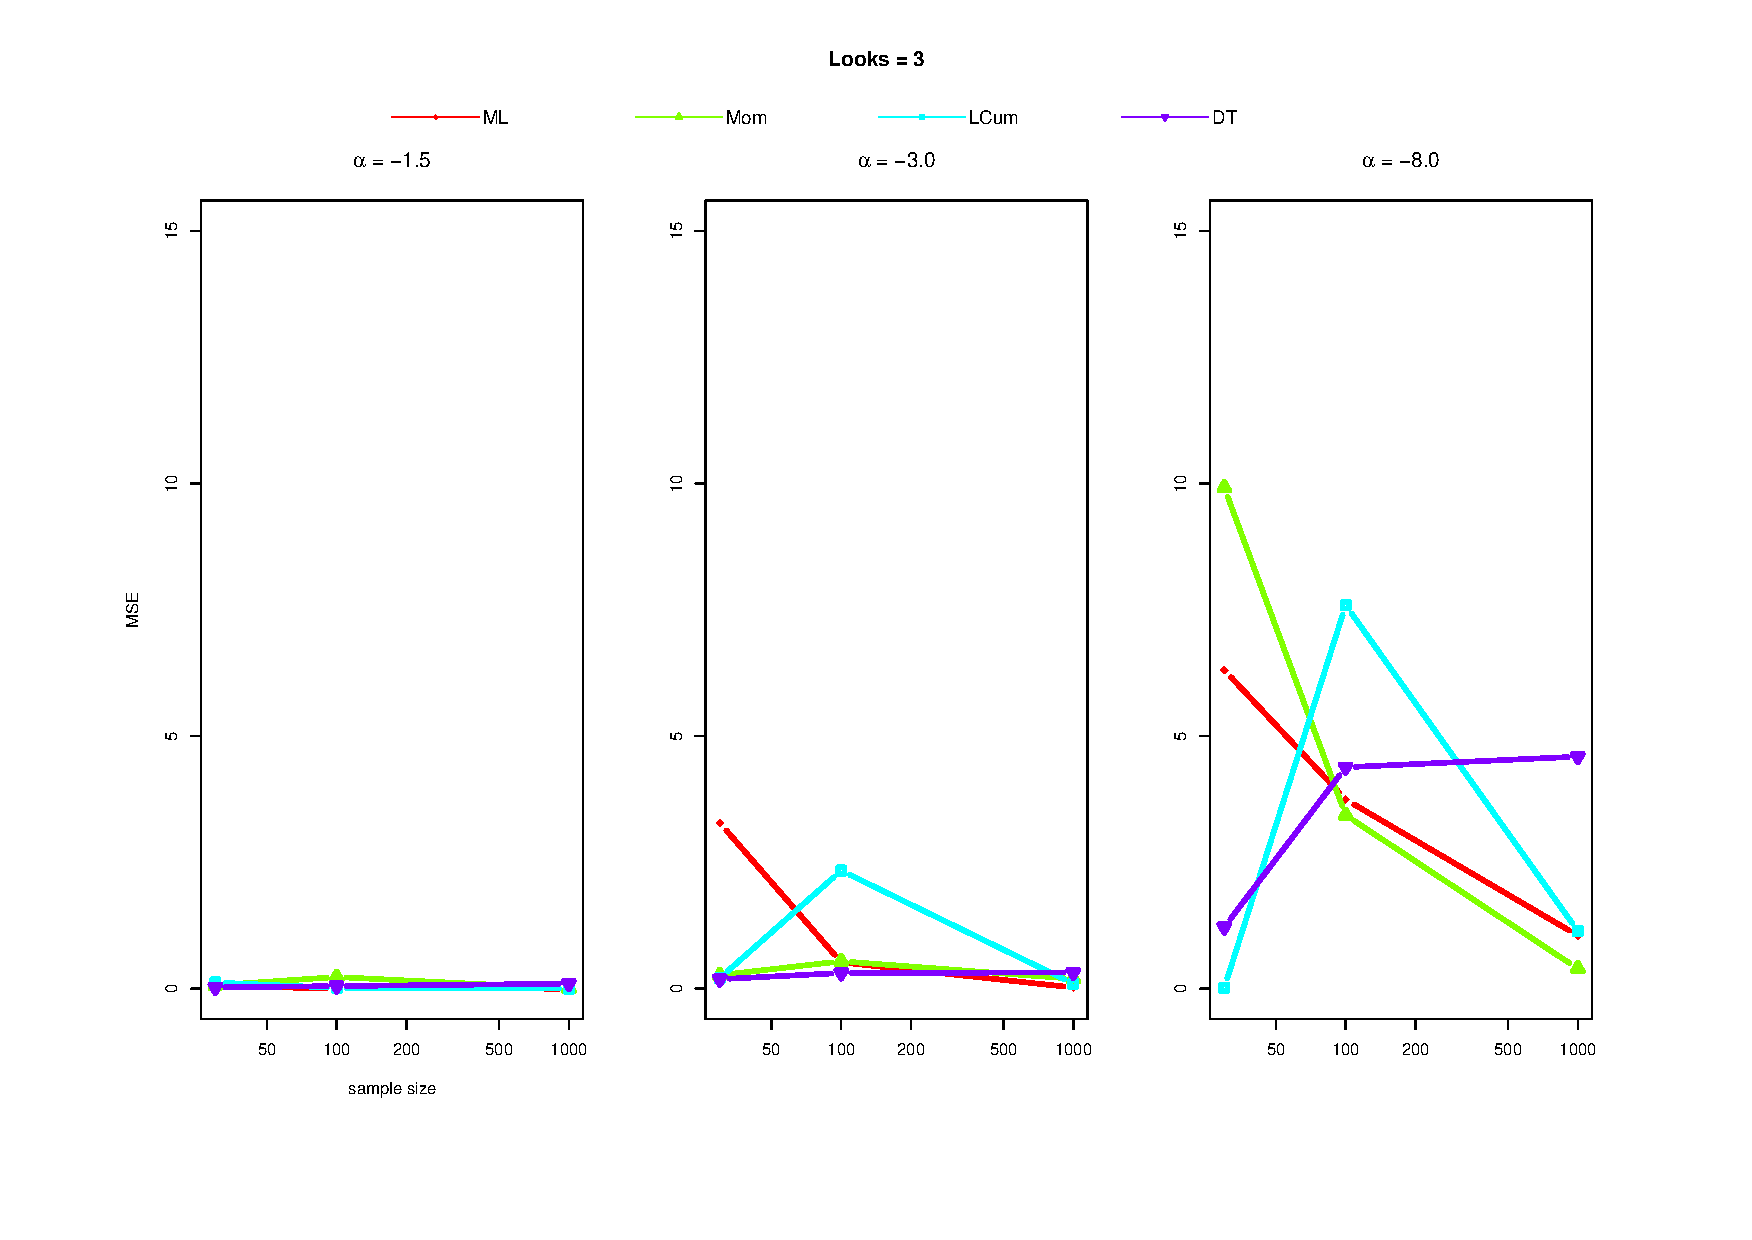
\includegraphics[scale=0.45]{plots/mse_L=3.pdf}
     \caption{Erros obtidos para $L=3$}
     \label{graf_13}
\end{figure}
\begin{figure}[H]
     \centering
     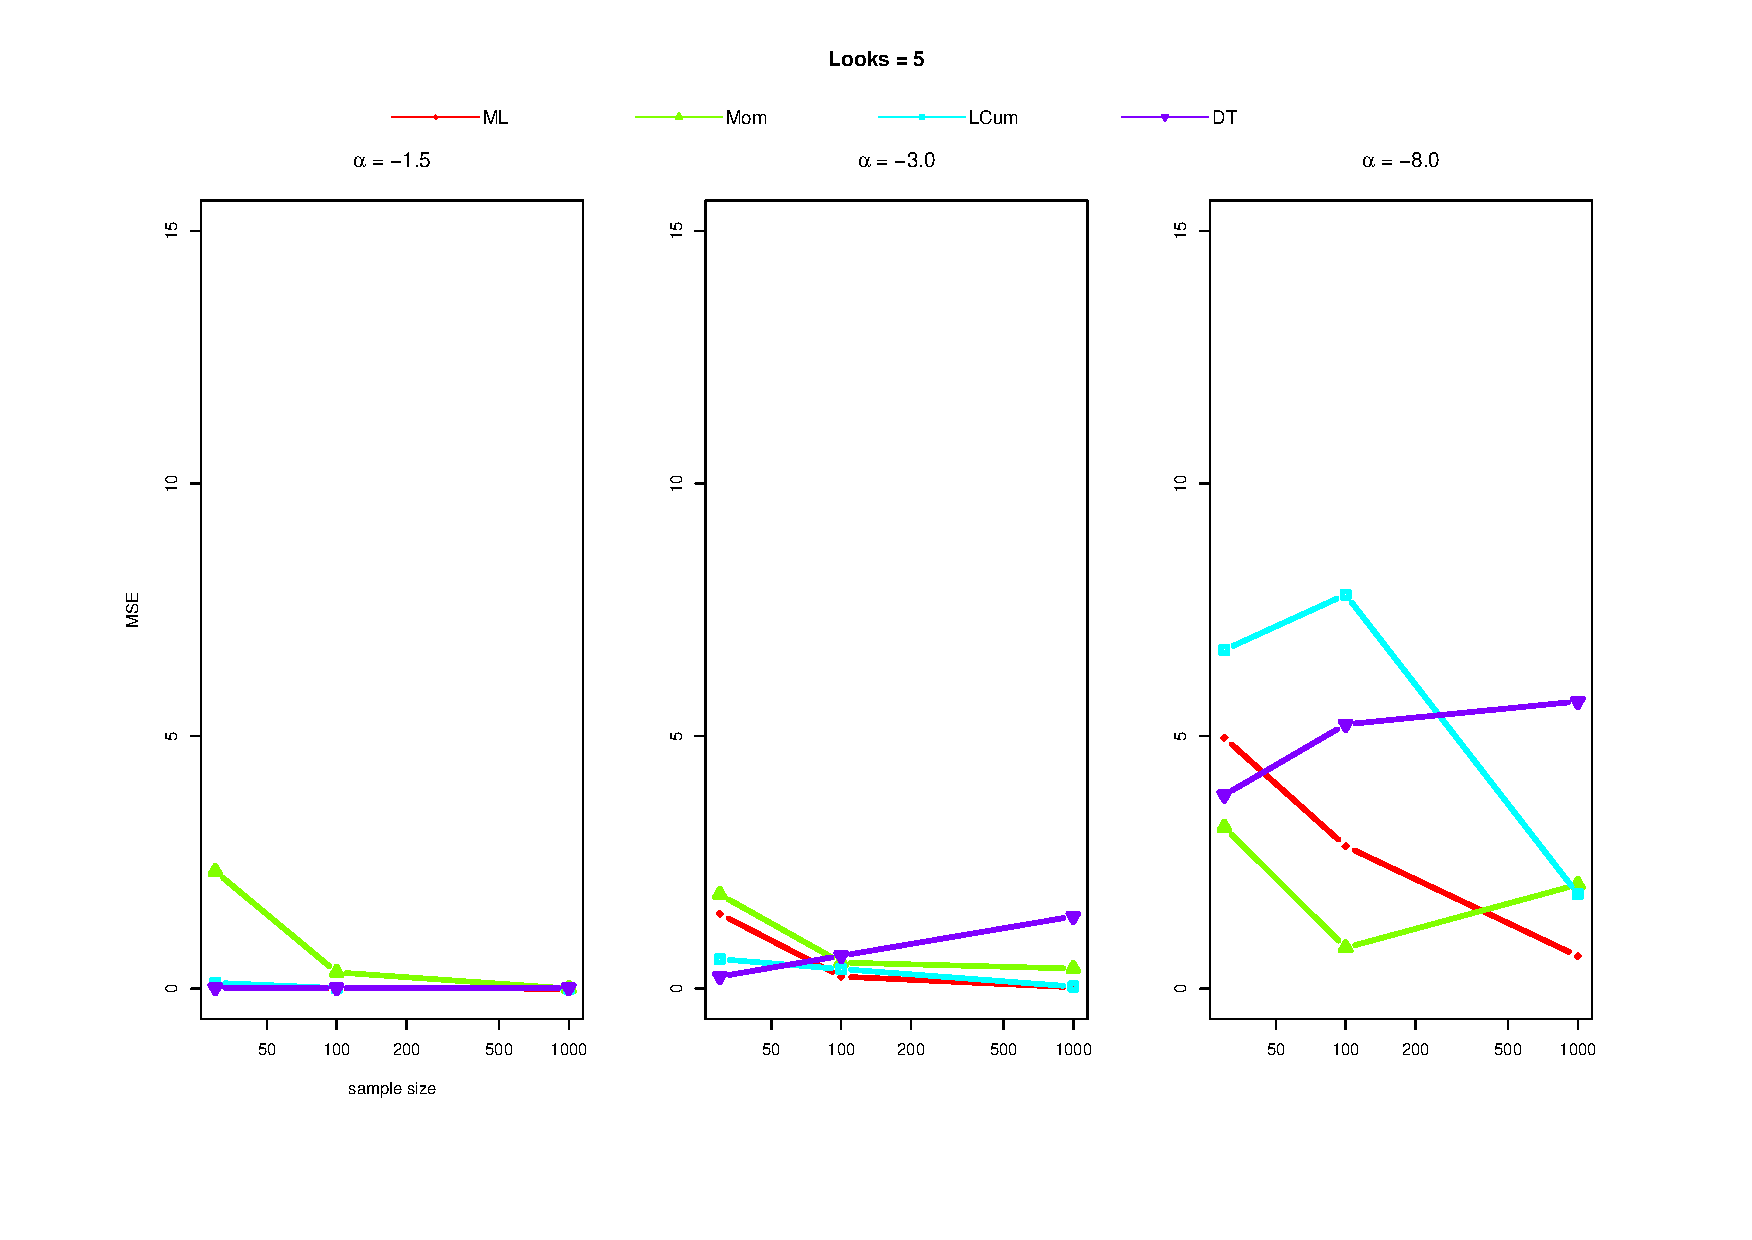
\includegraphics[scale=0.45]{plots/mse_L=5.pdf}
     \caption{Erros obtidos para $L=5$}
     \label{graf_14}
\end{figure}
\begin{figure}[H]
     \centering
     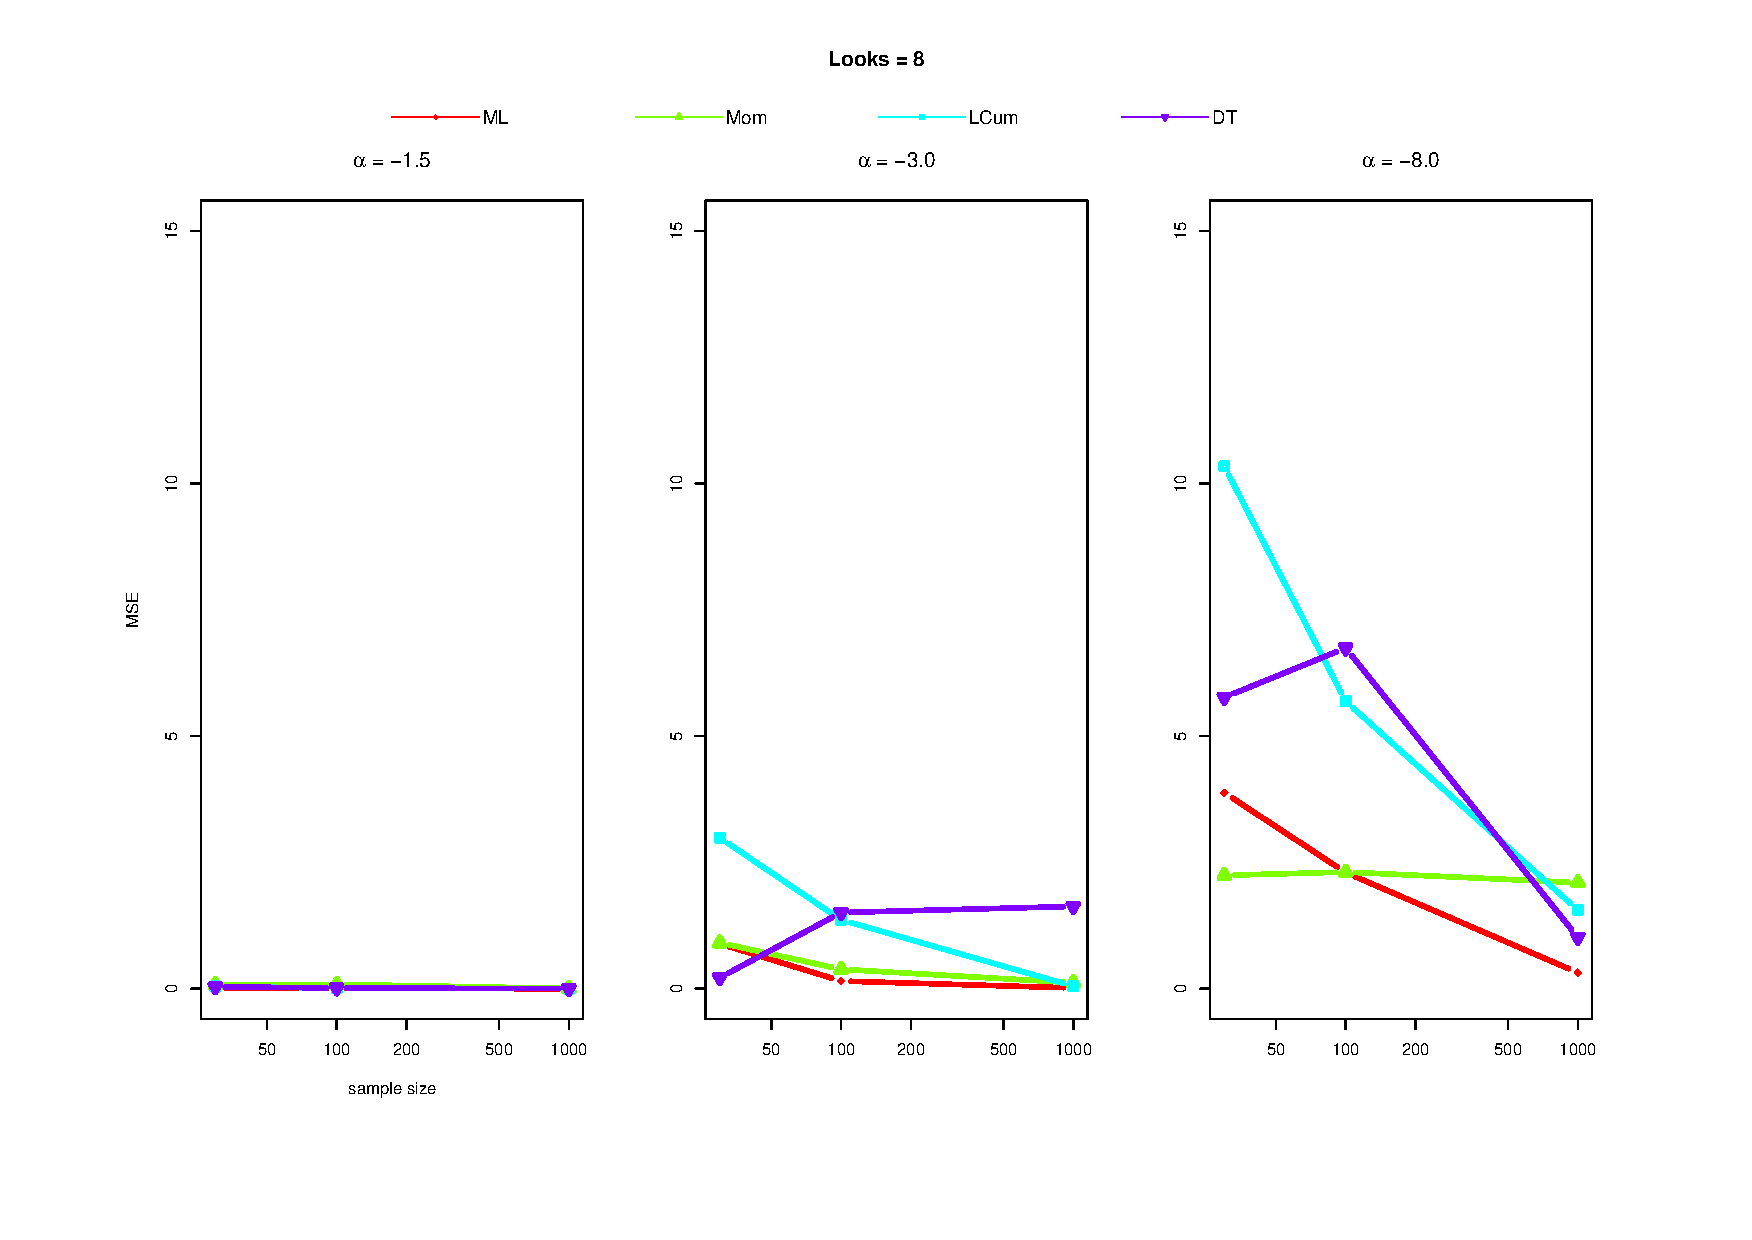
\includegraphics[scale=0.45]{plots/mse_L=8.pdf}
     \caption{Erros obtidos para $L=8$}
     \label{graf_15}
\end{figure}

Ao analisar todos os gráficos gerados, podemos perceber que duas técnicas de estimação apresentam, em média, estimadores muito próximos do valor verdadeiro: Máxima Verossimilhança e Distância Triangular. Os gráficos ainda mostram que para valores de $\alpha$ cada vez menores, independentemente do número de \textit{Looks}, as estimativas vão se tornando cada vez discrepantes em relação ao valor verdadeiro. É bastante notável a discrepância dos estimadores de Momentos e Log-Cumulantes quando $\alpha = -8$, e, mais especificamente, quando $L = 1$. 

Não obstante, é perceptível que 
$\widehat{\alpha}_{ML}$ tem uma tendência sistemática para subestimar o verdadeiro valor de $\alpha$. Além dessas observações, vale salientar que para o valor de $\alpha = -1.5$ as estimativas providas por todas as técnicas se mostraram bem próximas do valor verdadeiro do parâmetro em questão. \citet{FreryStochasticDistances2015} calcularam uma aproximação de primeira ordem de tal viés para um modelo estreitamente relacionado, e os resultados obtidos aqui estão de acordo com aqueles.

Vale ressaltar ainda que há possibilidade de uma eventual falta de convergência inerente a todos os algoritmos de estimação, visto que nem sempre tais algoritmos são extremamente precisos no cálculo e/ou podem falhar resultando em estimadores bem discrepantes do valor real ou simplesmente não conseguir encontrar a solução, devido, por exemplo, a não existência de raízes das equações lineares que os algoritmos de Momentos e Log-Cumulantes utilizam ou a falha na otimização dos algoritmos de Máxima Verossimilhança e Distância Triangular.

Ademais, nas figuras acima, onde estão mostrados os gráficos com os erros quadráticos médios referentes à cada técnica de estimação, pode-se perceber que, na maioria dos casos, todos os estimadores têm erro quadrático médio (\textit{mse - mean square error}) muito semelhante, não sendo possível afirmar com certeza que um deles é sistematicamente o melhor que o outro. O que pode ser feito é analisar onde cada estimador pode ser melhor aplicado observando os casos em que os mesmos obtiveram os melhores resultados e possuem menores chances de fornecer más estimativas. É baseado nessa ideia de construção de um algoritmo de estimação integrado com todos os algoritmos de estimação que esse trabalho propôs a criação de uma rotina de estimação unificada que encapsula diversos desses métodos e seja capaz de escolher o melhor para cada caso que lhe aparece. Essa rotina será melhor explicada na seção seguinte.

\section{Rotina de Estimação Unificada}

\subsection{Considerações iniciais}

Esta seção visa abordar o funcionamento geral da rotina de estimação que encapsula os algoritmos de estimação implementados e tem autonomia para tomar alguma decisão e executar alguma das técnicas desenvolvidas, diante de cada situação prevista. 

Com base nos experimentos de Monte Carlo que foram realizados foi possível fazer uma avaliação geral da qualidade de cada técnica implementada analisando o desempenho de cada uma delas em diferentes cenários considerando diferentes números de \textit{Looks}, diferentes graus de textura da imagem --homogênea, heterogênea ou extremamente heterogênea-- e diferentes tamanhos de amostra. 
O funcionamento de tal rotina de estimação foi pensado com base na análise de estudos feitos na literatura e, sobretudo, com base nos experimentos realizados.

Na subseção seguinte temos o fluxograma do funcionamento geral da rotina de estimação implementada, bem como algumas explicações e diretrizes, escritas em detalhes, que foram tomadas para a sua construção. 

\subsection{Fluxograma de Execução da Rotina de Estimação}

A figura~\ref{fig_fluxograma} apresenta o fluxograma de execução propriamente dito. Como pode-se perceber, a rotina de estimação desenvolvida é tolerante a falhas. Tolerância a falhas é a propriedade que permite que sistemas computacionais ou outros tipos de sistemas continuem a operar normalmente mesmo após ocorrência de falhas em alguns de seus componentes, seguindo, nesse caso, um fluxo de execução alternativo. Nesse sentido, a rotina desenvolvida sempre vai tentar retornar para o usuário um valor para o estimador, independente de falha em algum algoritmo, a não ser que a entrada de dados definida por ele seja inválida. O seguinte raciocínio foi levado em consideração para a construção desse fluxograma:
\begin{itemize}
    \item No início temos a interação com o usuário onde o mesmo tem a opção de escolher um algoritmo em especial para executar a estimação ou então não indicar opção alguma (opção nula) e deixar o sistema escolher a mais apropriada para cada caso.
    \item Se foi escolhido um algoritmo específico, o sistema vai tentar executar esse algoritmo e, se não ocorrer falhas, retorna o estimador calculado. Se houver falha, o sistema também saberá como agir verificando o tamanho da amostra e seguindo adiante até a execução de outro estimador.
    \item Se não foi escolhido um algoritmo específico ou se houver falha no passo anterior, há a verificação do tamanho da amostra da entrada. Se $n$ < $200$, parte-se para o método de Log-Cumulantes que se mostrou apropriado para trabalhar com amostras pequenas. O sistema vai tentar executar esse método e, se não houver falhas, retorna o estimador calculado. Se houver falha, parte-se para a verificação do número de \textit{Looks} e o sistema segue adiante até a execução de outro estimador.
    \item Se o tamanho da amostra for maior ou igual que $200$ ($n \geq 200$) ou se houver falha no passo anterior, há a verificação do número de \textit{Looks}. No caso em que $L \leq 5$ executa-se a estimação por Máxima Verossimilhança que forneceu resultados bem precisos nesse caso e o estimador é calculado, se não houver falhas. Se falhar, parte-se para a verificação da textura da região.
    \item No caso em que temos $L$ > $5$ ou se houver falha no passo anterior, faz-se a verificação da textura por meio do parâmetro $\alpha$. A estimação por Distâncias Estocásticas utiliza métodos de minimização que são mais estáveis e possuem menor erro nos casos em que temos um número grande de \textit{Looks} e valores próximos de zero do parâmetro $\alpha$ que correspondem a regiões extremamente rugosas da imagem, conforme aborda \citet{Cassetti2013} em seu trabalho. Assim, o sistema vai tentar executar esse algoritmo de Distâncias Estocásticas e exibir o resultado. Se houver falhas, parte-se para o método dos Momentos. 
    \item Por sua vez, o método dos momentos vai ser executado no caso em que o parâmetro $\alpha \leq -3$ ou se houver falha no passo anterior e, caso não ocorra falhas, o resultado será exibido. Se houver falhas, executa-se a estimação pelo algoritmo de Máxima Verossimilhança (foi o que apresentou os melhores resultados no geral) e exibe-se o resultado. Se esse algoritmo falhar, exibe-se a mensagem de erro para o usuário e solicita-se para o mesmo tentar novamente com dados válidos.
\end{itemize}
%%% ACF Verifique por que < e > não aparecem no PDF

\begin{figure}[H]
     \centering
     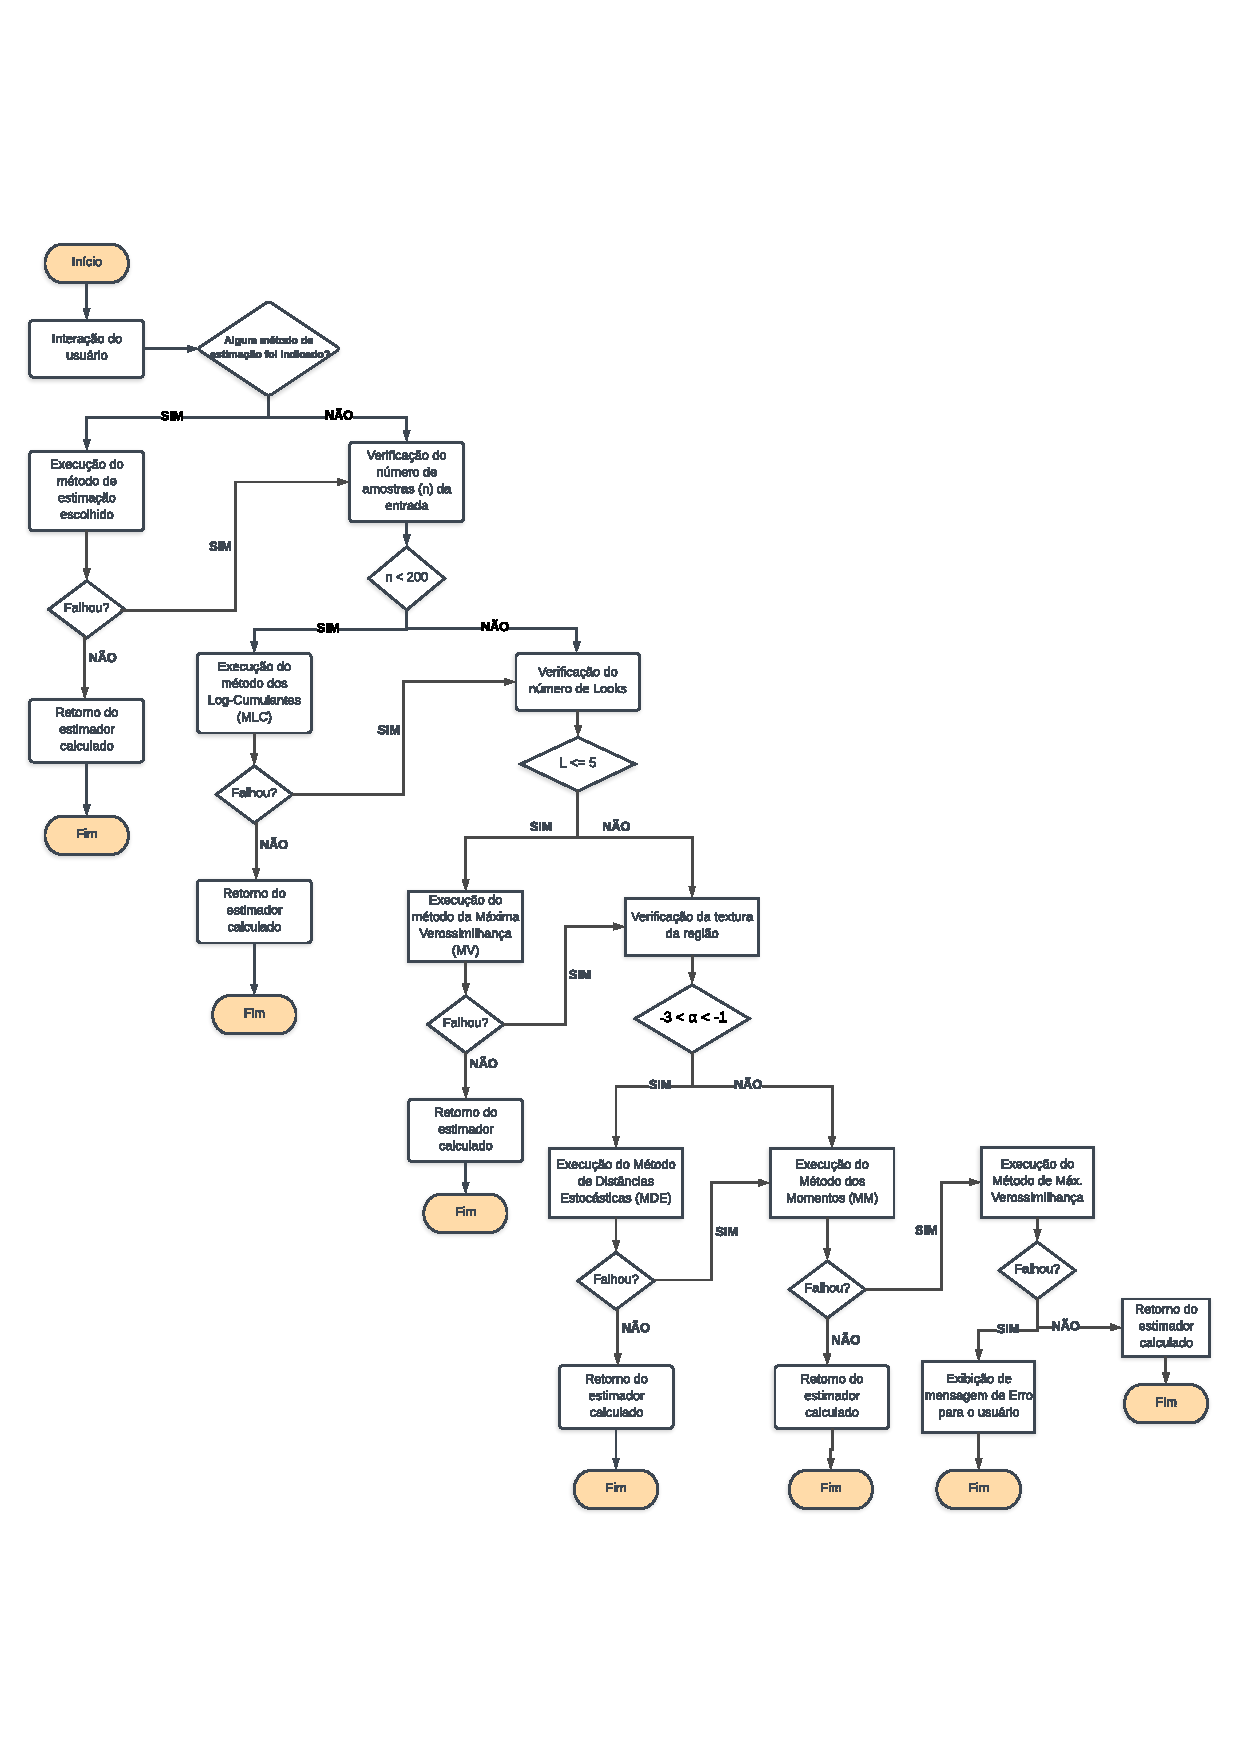
\includegraphics[width=\linewidth]{plots/FluxogramaDeExecucao-A4.pdf}
     \caption{Fluxograma de execução da rotina de estimação}
     \label{fig_fluxograma}
\end{figure}

